\documentclass[a4paper]{article}
\usepackage[utf8]{inputenc}
\usepackage{float}
\usepackage{pdfpages}
\usepackage{textcomp}
\usepackage{indentfirst}

\setlength{\parskip}{1em}

% Colour Management
\usepackage{color}

% Multi-Line Comments
\usepackage{comment}

% Customisable Sections
\usepackage{titlesec}
\titleformat{\paragraph}[hang]{\normalfont\normalsize\bfseries}{\theparagraph}{1em}{}
\titlespacing*{\paragraph}{0pt}{3.25ex plus 1ex minus .2ex}{1em}

% Images and Captions
\usepackage{graphicx}
\usepackage{subcaption}
\usepackage{wrapfig}
\graphicspath{{./images/}}
\usepackage{fancyhdr} 


% Bibliography
\usepackage[nottoc]{tocbibind}
\usepackage[
    backend=biber,
    sorting = nty, 
    style=ieee]{biblatex}

\addbibresource{report_citations.bib} %Imports bibliography file

\usepackage{amsmath} %sudo tlmgr install amsmath


% Tables
\usepackage{array}
\newcolumntype{L}{>{\raggedright\arraybackslash}m{0.9\linewidth}}
\usepackage{ragged2e}
\usepackage{hhline}
\usepackage{multicol}
\usepackage[outdir=./media]{epstopdf}

% Contents Page
\usepackage{hyperref}

% Appendices
\usepackage[toc,page]{appendix}

% Bold Maths Symbols
\usepackage{bm}
\usepackage{gensymb} %sudo tlmgr install was
\usepackage{multicol}

%Command for adding units to equations
\newcommand{\unit}[1]{\ensuremath{\, \mathrm{#1}}}


% Allowing lower levels of Contents Page
\setcounter{tocdepth}{4}
\setcounter{secnumdepth}{5}

% Make margins smaller, feel free to change
\usepackage{geometry}
\geometry{
    a4paper,
    top = 20mm,
    bottom = 20mm,
    textwidth=450pt
}





\title{Engineering Design Project}
\author{Georgios Chaimali \and 
        Dimitrios Georgakopoulos \and 
        Edvard J. Skaarberg Holen \and 
        Hyunjoon Jeon \and 
        Josiah Mendes \and 
        Raghav Viswakumar}
\begin{document} 
\begin{titlepage}
    \setlength{\headheight}{66.89pt}
    \thispagestyle{fancy}
    \renewcommand{\headrulewidth}{0pt}
    \renewcommand{\footrulewidth}{0pt}
    \lhead{
\includegraphics[scale=0.1]{logo.png}}
    \cfoot{} % this is to remove the page number
    \hbox{}\vfill
    \begin{center} 
	    {\scshape\LARGE Imperial College London  \par}
	    \vspace{1cm}
        {\scshape\Large Second Year Design Project\par}
        \vspace{0.25cm}
        {\scshape\Large ELEC50003/ELEC50008\par}
        \vspace{1.5cm}
        {\huge\bfseries The MARS Rover\par}
        \vspace{2cm}
        {\Large\itshape Group 1\par}
        \vfill
        \begin{flushright}
            \textsl{ \large
            Georgios Chaimali \\ 
            Dimitrios Georgakopoulos \\ 
            Edvard J. Skaarberg Holen \\ 
            Hyunjoon Jeon \\ 
            Josiah Mendes \\ 
            Raghav Viswakumar
            }
        \end{flushright}
        \vfill

        % Bottom of the page
        {\large Word Count: XXXX Words \\ \today\par}
        \vfill
    \end{center}
\end{titlepage}
 
\setcounter{tocdepth}{2}
\tableofcontents

\newpage

\section{Introduction}

\section{Structural Design}

\section{Functional Design}

\subsection{Control}
\subsubsection{Requirements}
\subsubsection{Initial Design Choices} 

\subsection{Command}
\subsubsection{Requirements}
\subsubsection{Initial Design}

\subsection{Drive}
\subsubsection{Requirements}
\subsubsection{Initial Design}


\subsection{Integration}
\subsubsection{Requirements}
\subsubsection{Initial Design}
\subsection{Command}

\subsubsection{Purpose of the module}

The Command module has three main purposes within the system of the rover:

\begin{enumerate}
    \item Visualise data from the other subsystems
    \item Allow users to command the rover
    \item Calculate paths for the rover to follow based on the commands given by the users
\end{enumerate}

In order to achieve the aforementioned goals, it was important to establish connection between the Command 
module as a server, and other subsystems as clients. The ESP32 of the Control module is the main client 
that constantly communicates with the server to exchange commands and status of the rover. The energy module 
is another client and regularly sends data related to the battery of the rover. The received data are presented 
on a web application where users can check the current status of the rover and command the rover. In order to 
smoothly handle incoming data and render components that form the web application, the web application was divided 
into the server-side, backend, and the presentation side, front end, written in Node js and React respectively.

\subsubsection{Communication with Control}

\subsubsection{Communication with Energy}
Similar to the connection with the Control module, the Command module communicates with the Energy module over 
the TCP protocol. 

\subsubsection{Communication between Backend and Frontend}
A reliable connection between the backend and the frontend during the rover's operation is necessary for the web 
application because users would interact with the frontend only while path calculations and communication with 
the rover would be done on the backend. For this reason, certain data have to be shared between the server 
and application side. There are multiple communication protocols available and although the HTTP protocol was used 
in the beginning of the project, WebSocket was considered to be more suitable and advantageous as the project 
progressed. 

The HTTP protocol is uni-directional. This means that the connection can be established only from one side between the 
server and clients. In case of the frontend-backend connection, the backend could send data to the frontend as a response 
only when it received a request from the frontend. This aspect of the HTTP protocol was not so convenient when the 
backend 

\subsubsection{A* Algorithm}

\subsection{Vision}
The purpose of the Vision module is threefold:
    1. Capture data from camera module;
    2. Detect objects of interest within the current view, namely 5 different
    coloured table-tennis balls and 
    send their location to the Control module; and
    3. Send image data to Control for streaming to Command. 


\subsubsection{Initial Design Choices}


%Start of functional energy section
\subsection{Energy}
\subsubsection{Requirements}

The main goal of the energy sub-module is to design a battery pack for the 
rover and charge it using solar power. With this goal in mind, the energy 
sub-module must develop a battery management system which allows the tracking 
of battery SOC and SOH, and if necessary perform SOH maintenance.         


\subsubsection{Characterising Components}
When designing a system it is necessary to know the behaviour and limitations of its
constituent components. There are three main components that make up the energy 
subsystem: the battery cells, the PV panels and the SMPS.

\paragraph*{Battery Cells}
To determine the behaviour of the battery cells they were all tracked through a full charge/discharge 
cycle using the provided “Battery\_Charge\_Cycle\_Logged\_V1.1.ino” code\cite{chargeCode}. 
Every cell behaved similarly in terms of the cell voltage compared to time. 
The cell voltage of cell 1 over a full discharge/charge cycle is shown in Figure~\ref{fig:charge_cycle}:

\begin{figure}[H]
    \centering
    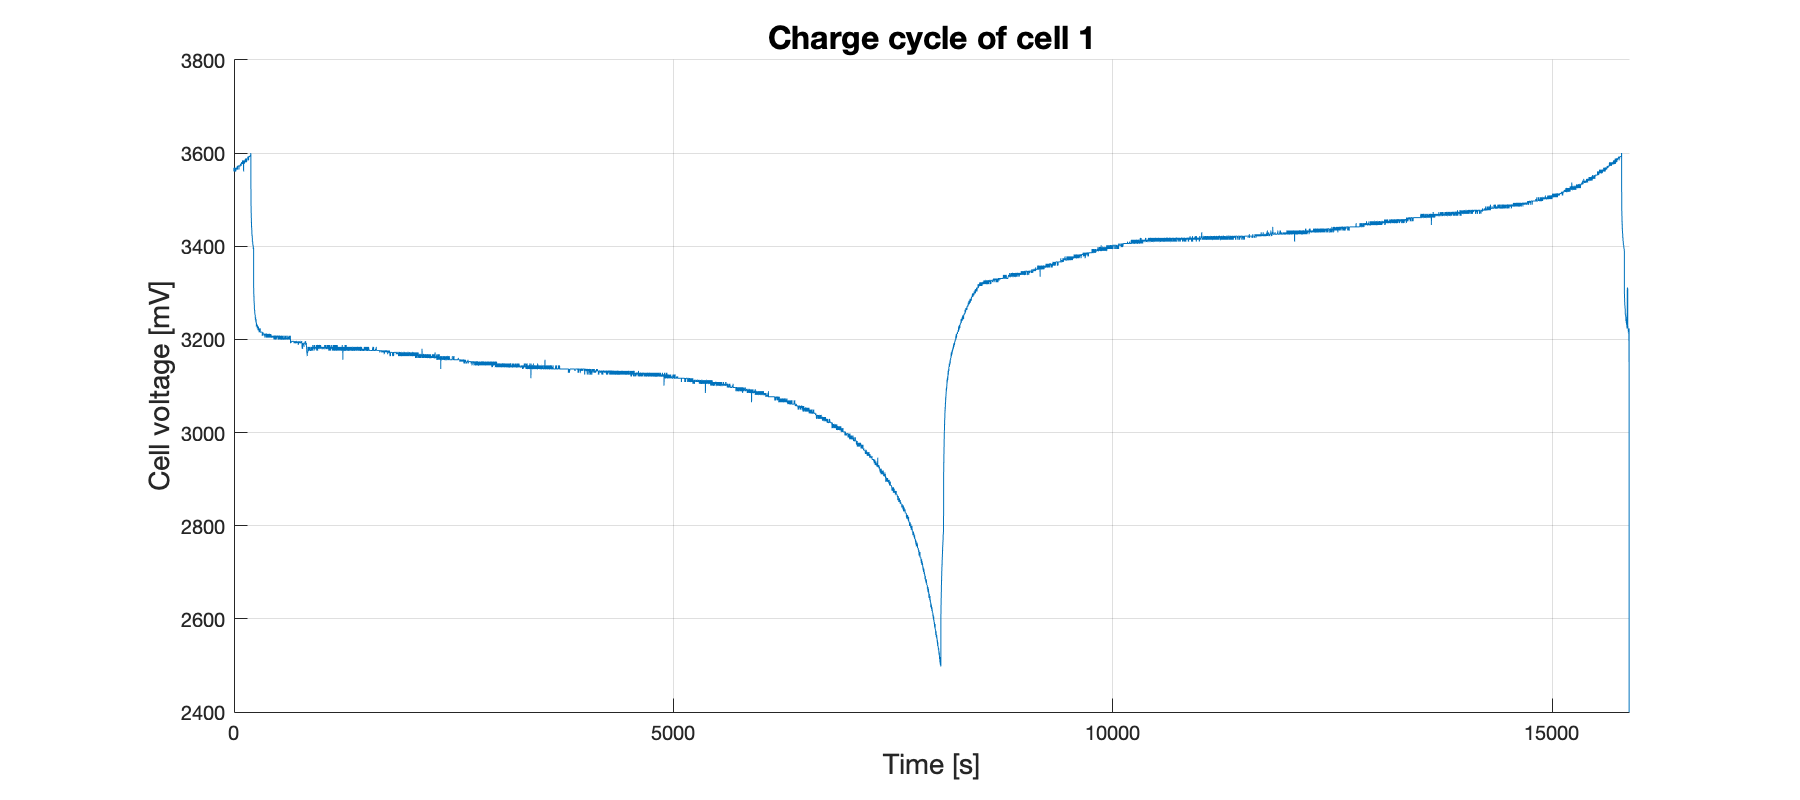
\includegraphics[scale=0.18]{charge_cycle.png}
    \caption{The voltage evolution of cell 1 through a full discharge/charge cycle.}
    \label{fig:charge_cycle}
\end{figure}

Note the following important points on the graph. At 200 s the cell is done charging and
enters an idle state for 30 s after which it starts discharging. At ~8000 s the cell is fully
discharges and enters an idle state for 30s after which it starts charging. Finally, at 18800 s the cell is once 
again fully charged and the charge cycle is completed.

The provided charging algorithm also logs the current into the cell.
By integrating said current for a full charge or discharge section
we can determine the cell capacity in mAh. The results of this analysis is 
presented in the table below:

\begin{center}
    \begin{tabular}{||c| c c c c c||} 
    \hline
    Cell Number& 1 & 2 & 3 & 4 & 5 \\ [0.5ex] 
    \hline
    Capacity (mAh) & 542.7	& 526.1	& 519.5	& 530.1	& 543.7\\ [1ex] 
    \hline
    \end{tabular}
    \end{center}


As expected all cells have a capacity somewhere around 500 mAh. However, some cells
are have a higher capacity than others which may have implications for the performance
of certain battery cell configurations.

\paragraph*{PV panels}
The provided PV panels are rated for a maximum power of 1.15 W at a voltage 
of 5.0 V and current 230 mA. Away from the maximum power point the performance of 
the panels can be determined from their I-V curves. To find the I-V curves each 
panel was connected to the B-inputs of the SMPS operating in non-synchronous boost.
They were then lit by the lamp and the duty cycle of the SMPS was varied while measurements 
of panel current and voltage were taken. After processing the resulting data
is plotted in Figure~\ref{fig:IV_curve}.

    \begin{figure}[H]
    \centering
    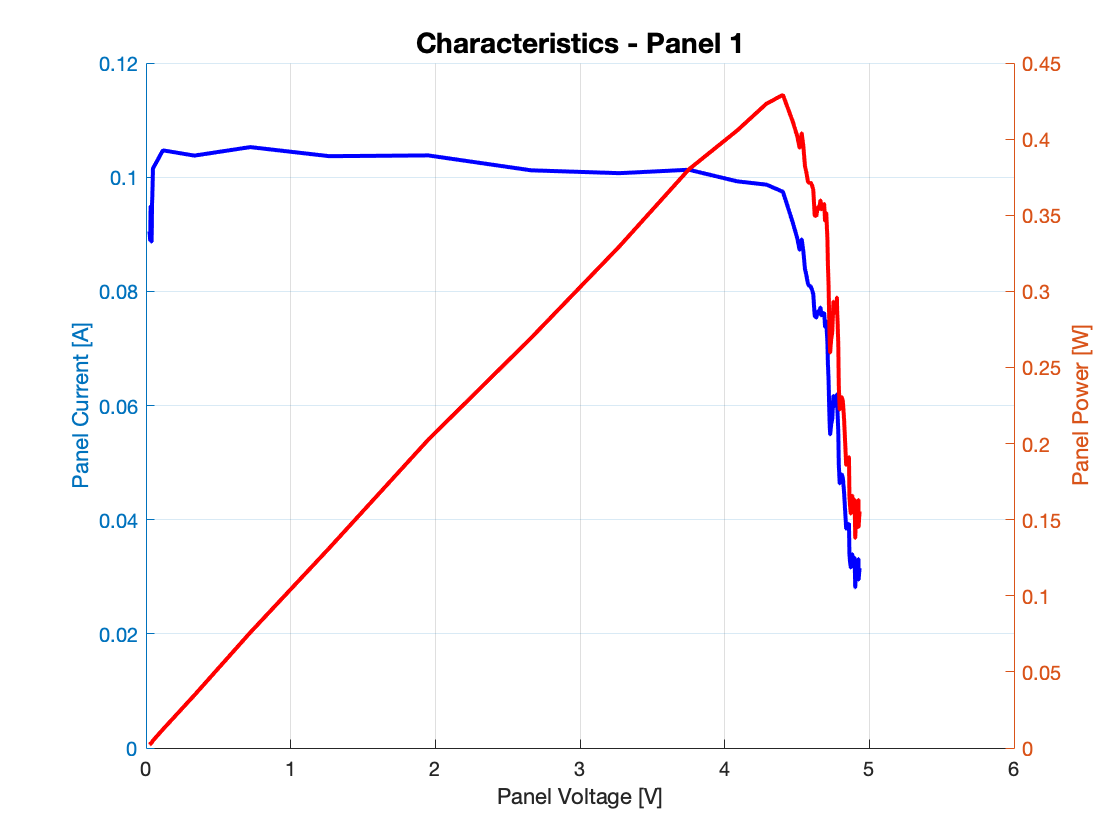
\includegraphics[scale=0.18]{Panel1.png}
    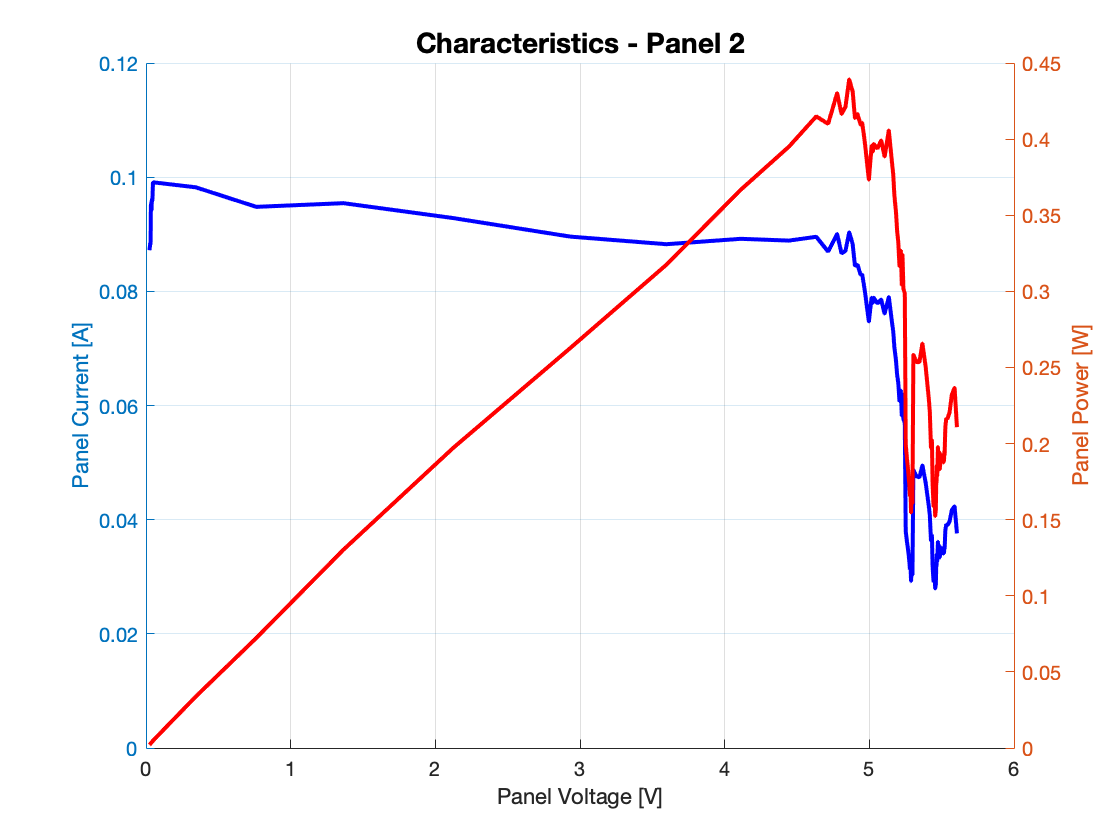
\includegraphics[scale=0.18]{Panel2.png}
    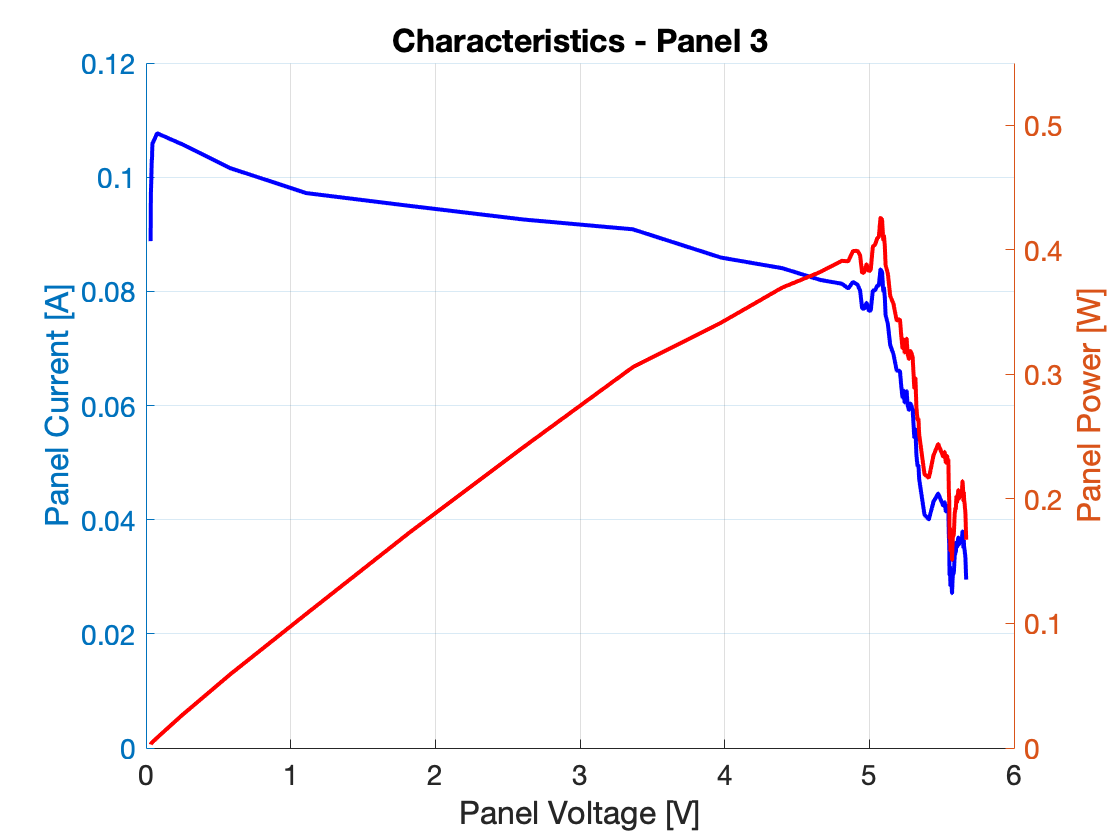
\includegraphics[scale=0.18]{Panel3.png}
    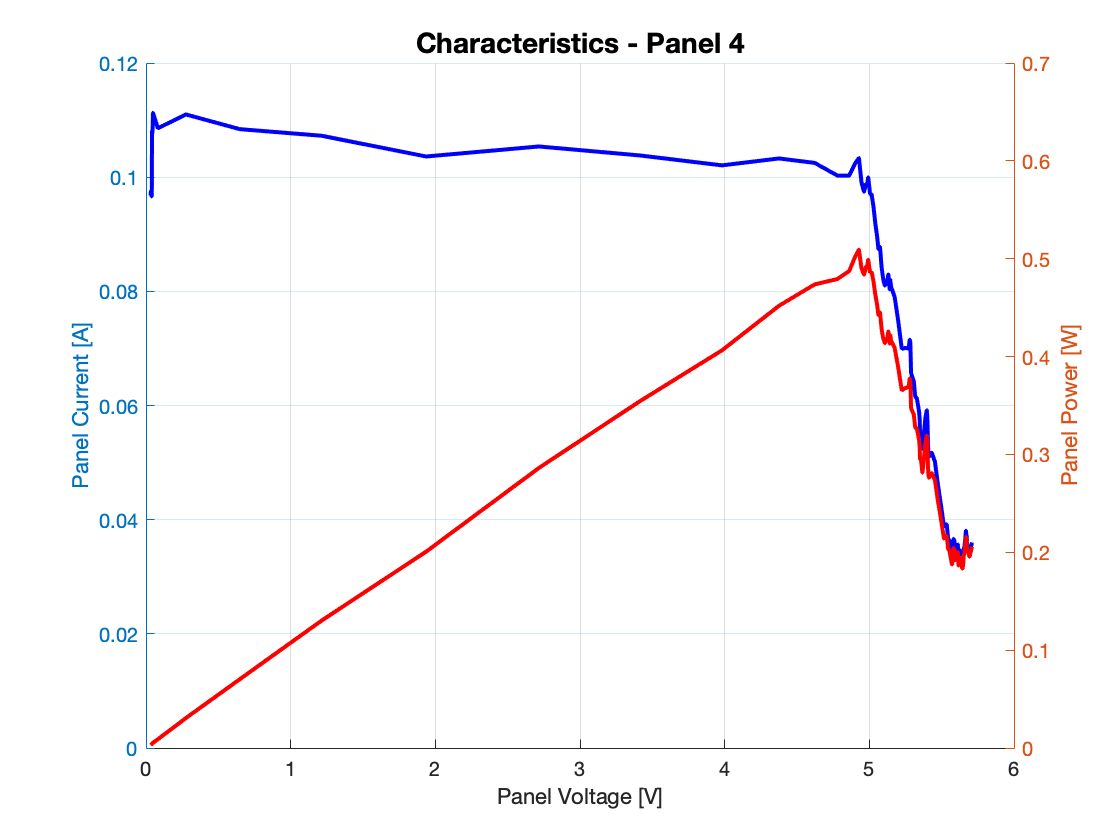
\includegraphics[scale=0.18]{Panel4.png}
    \caption{I-V curves for the PV panels.}
    \label{fig:IV_curve}
    \end{figure}

Though the data is noisy, it is clear that all panels exhibit the standard 
I-V characteristics of a PV cell. That is, they behave as non-ideal current 
sources with a nearly constant current at low voltages and a rapid current 
reduction at high voltages\cite{green}. Moreover, we see that the provided lamp activates 
the panels poorly as the peak power for each of the panels is only ~0.5 W.

\paragraph*{SMPS}
\begin{wrapfigure}[16]{r}[0pt]{0.5\textwidth}
    \centering
    \raisebox{0pt}[\dimexpr\height-3\baselineskip\relax]{%
        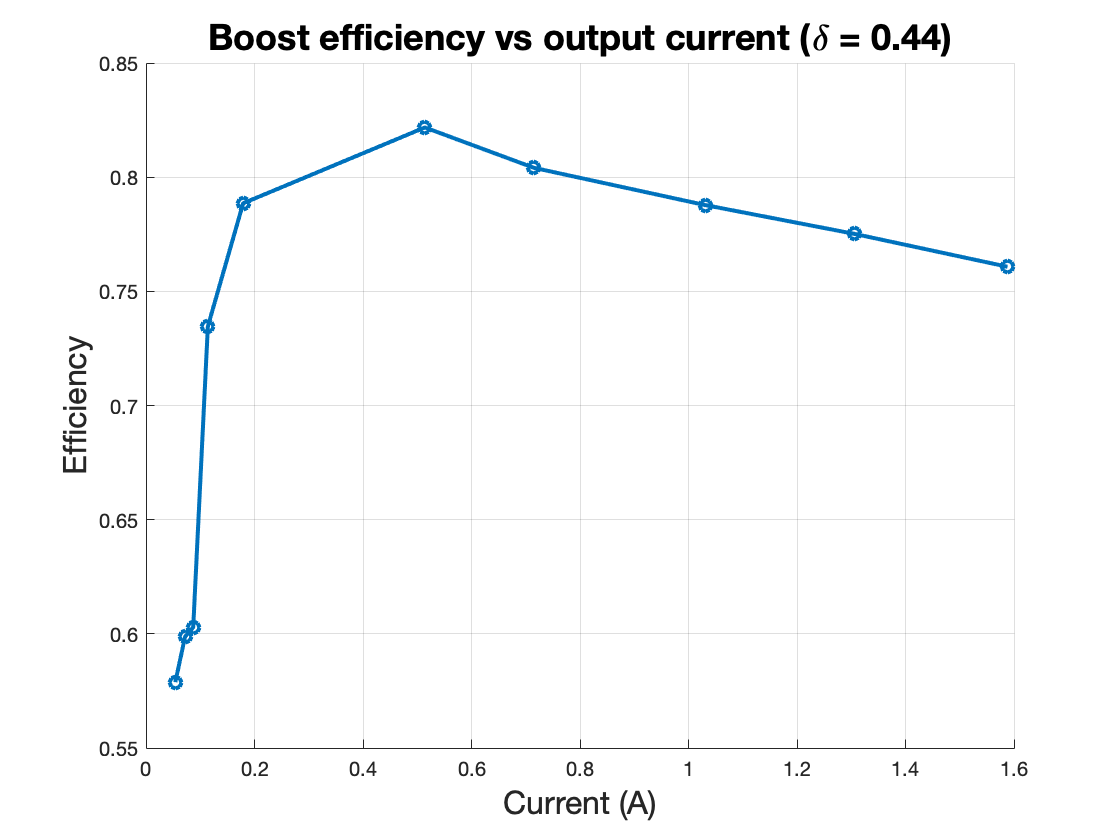
\includegraphics[width=0.48\textwidth]{Boost_efficiency_wduty.png}
    }%
    \vspace{0pt}
    \caption{SMPS efficiency versus output current with input voltage 5V [reference to logbook]}
    \label{fig:efficiency}
\end{wrapfigure}
The provided SMPS is rated for 10 W throughput with a maximum boost output voltage of 35 V 
and maximum output current of 10 A\cite{SMPS_lab}. All these ratings are far higher 
than needed and neither is expected to impose limitations on the design of the energy module. 

The many characteristics of the SMPS have been thoroughly examined in 
2nd year labs. However, for the energy submodule the most important characteristics 
will be the SMPS efficiency during non-synchronous boost operation. A graph of 
efficiency versus output current is shown in Figure~\ref{fig:efficiency}.


\subsubsection{Initial Design}

\textbf{Battery Configuration}
\vspace{10pt} 
\newline
When designing the battery pack there are two principal choices that need to be made. 
Firstly, how many battery cells should the battery pack consist of and, secondly, 
in what manner should these cells be connected? 

The optimal number of cells is in large part set by the energy 
and power needs of other submodules. During testing the total power 
draw of the rover was found to be about 2 W. Each battery cell has a 
nominal voltage of 3.2 V and a maximum peak discharge current of 1 A 
[battery datasheet], giving a maximum power draw of 3.2 W per cell. 
Thus, to meet the power requirements of the rover it is enough to use only 
one cell. However, each cell can only store about \(3.2 \unit{V} * 0.5 \unit{A} * 3600 \unit{s} \approx 5760 \unit{J} \), 
which would only power the rover for 48 minutes. It is desirable to have 
the rover be operational for as many hours as possible each day. 
Assuming that 12 hours a day are completely without sunlight it is clear 
that the rover cannot work through the night even if all 5 available 
battery cells were used. To give the rover the most operational hours we 
would then want to use all 5 battery cells. However, connecting 5 battery 
boards to the Arduino would use at least 11 of the 12 free Arduino pins, 
leaving only one pin for all other purposes. As such it might be wise to use 
less cells. To accommodate other circuit functions, only 4 cells will therefore be used.

Now consider the PV array. Each PV panel is rated for 1.15 W, meaning 
that the array as a whole should produce 4.6 W. As shown in Figure~\ref{fig:efficiency} the 
peak efficiency of the SMPS in boost mode is about 80\% giving a maximum 
usable power of \(0.8 * 4.6 \unit{W} \approx 3.7 \unit{W} \). Assuming 12 hours of sunlight in a day, 
this means that the PV array will produce less energy each day than the rover 
uses in 24 hours. It is therefore of high priority to capture as much of the 
solar power as possible. The battery cells have a standard charging current of 
250 mA \cite{batteryDatasheet}. The power needed to charge the at this current is 
shown in the table below:

\begin{center}
    \begin{tabular}{||c| c c c c c||} 
    \hline
    Number of cells& 1 & 2 & 3 & 4 & 5 \\ [0.5ex] 
    \hline
    Nominal charging power (W) & 0.8 & 1.6 & 2.4 & 3.2 & 4.0\\ [1ex] 
    \hline
    Peak charging power (W) & 0.9 & 1.8 & 2.7 & 3.6 & 4.5 \\ [1ex] 
    \hline
    \end{tabular}
\end{center}


A 4 cell battery pack is the largest battery pack which has a power 
requirement of less than 3.7 W at standard charging current and little 
power goes unused. Adding to this that the rover has most operational 
hours with 4 cells, using 4 cells is the clear choice. Note that the 
cells used are number 1, 2, 4 and 5 as these were found to have the 
highest capacity.

There are several ways to connect the 4 cells into a power pack, 
however the design brief advised against mixing parallel and series 
connections\cite{energyBrief}. As such only fully series and parallel 
battery packs will be considered. 

A series battery pack has some obvious disadvantages compared to 
a parallel battery pack. In section 2.5.1 it was shown that all the 
battery cells have different capacities. In a parallel battery pack 
this is not a big problem, as it is possible to draw different currents 
from each cell and thereby use the full capacity of each cell. For a 
series battery pack however, the total battery capacity will be limited 
by the cell with the lowest capacity. As such, a series battery pack 
is able to store less usable energy than an equivalent parallel battery 
pack. Moreover, to check the OCV of each cell they need to be switched 
out of circuit using the battery board relay. For a series battery pack 
this leads to an open circuit and any charging/discharging of the battery 
must halt while the voltage is measured. For a parallel battery pack on the 
other hand, switching the relay of a cell only takes that one cell out of 
circuit and it is possible to charge/discharge the battery pack while 
taking voltage measurements. Being able to switch single cells out of 
circuit can also enables switching faulty cells out of circuit, meaning 
that one cell failing would not mean that the battery pack as a whole fails. 
Finally, a parallel battery pack is self-balancing and energy automatically
flows between cells when necessary\cite{batteryBalancing}. Series cells on the 
other hand need to be balanced by switching on and off balancing resistor. 
This not only is more complex, but leads to power being lost in the balancing
resistors.

There is however one major weakness to a parallel battery pack: 
it is very hard to track the current going into individual cells. For 
safe operation it is necessary to prevent over-current into each individual 
cell. However, the current sensor on the SMPS can only measure the current 
flowing into the battery pack as a whole. Each battery cell is only rated 
for a rapid charging current of 500 mA\cite{batteryDatasheet},  and seeing 
as there is no way to know how the current splits into each of the cells 
one must operate one must operate with the assumption that all the current 
can flow into a single cell. As such, no more than 500 mA can be allowed 
to flow into the battery pack as a whole. At this current the nominal 
charge power is only \(3.2 \unit{V} * 0.5 \unit{A} = 1.6 \unit{W} \)
    meaning charging will be slow and it is only possible to use less than half of the available solar power. 
This is such a large drawback of using a parallel battery pack, that 
despite all the previously stated disadvantages of a series battery pack, 
a series battery pack has been deemed the best option.


\textbf{PV Array Configuration}
\vspace{10pt} 
\newline
To facilitate the highest power output all the four provided PV panels will be used.
There are four different ways in which the four panels can feasibly be connected. 
The different arrangements are shown in figure~\ref{fig:arrayConfigurations}.

\begin{figure}[H]
    \centering
    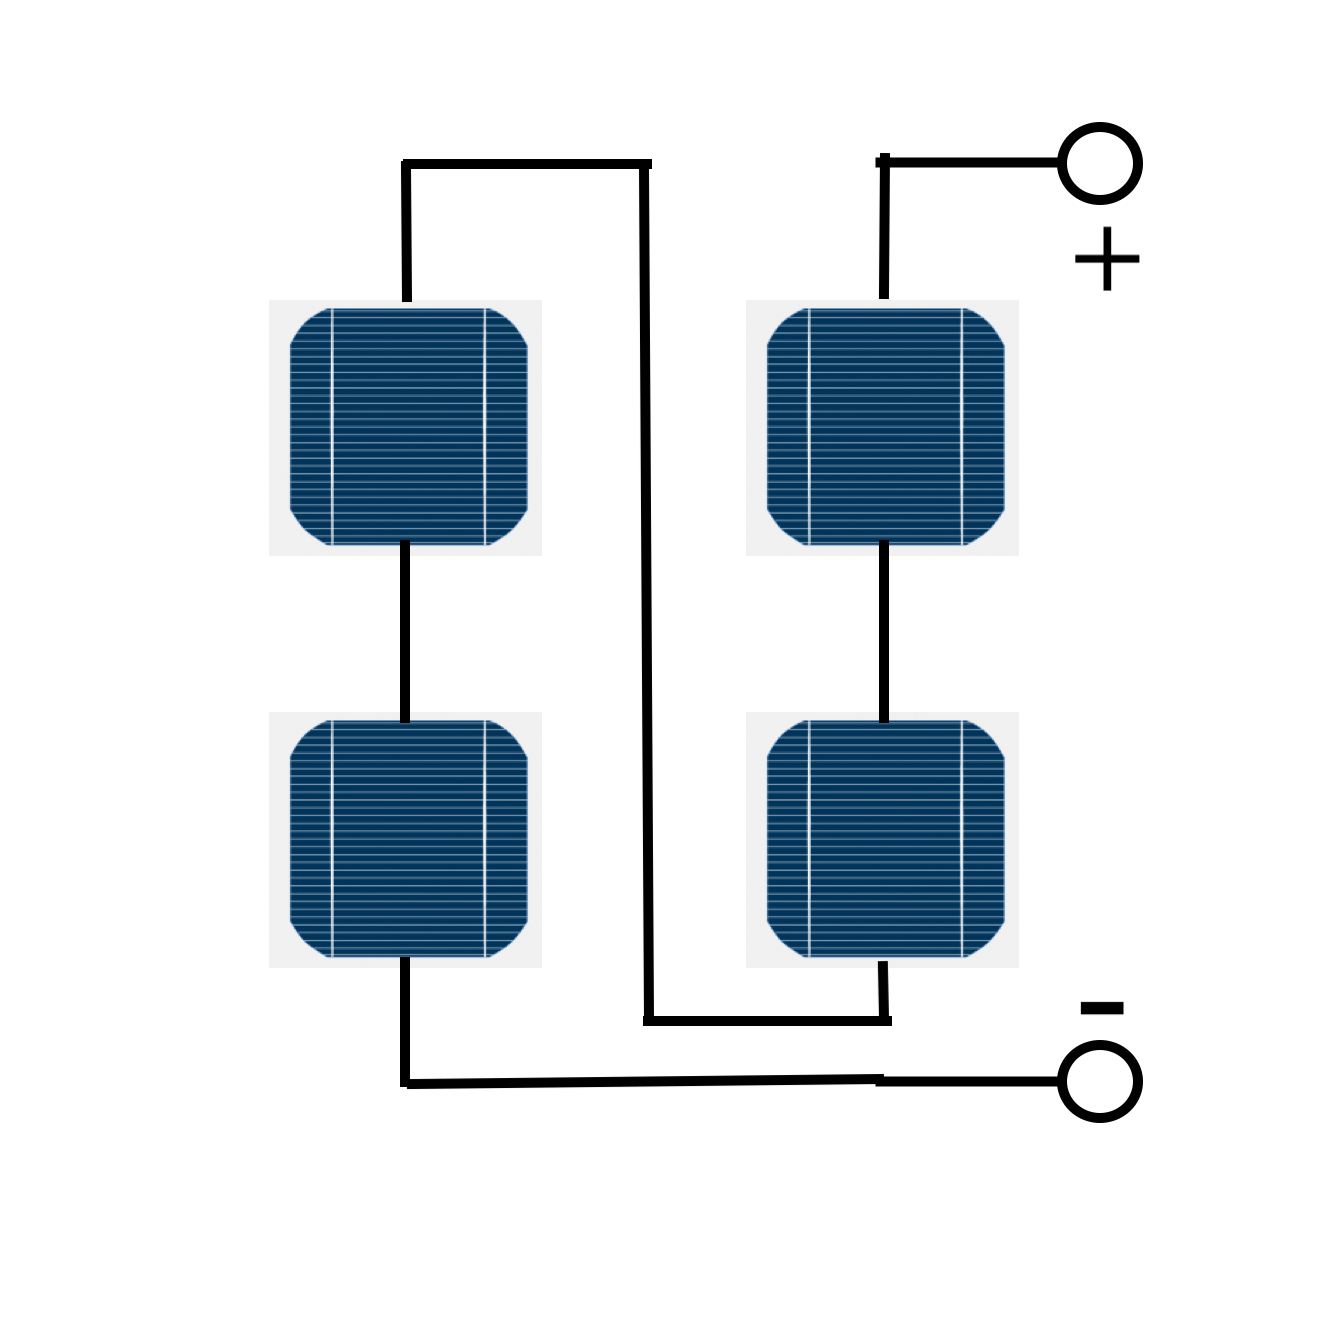
\includegraphics[scale=0.10]{Series(S)}
    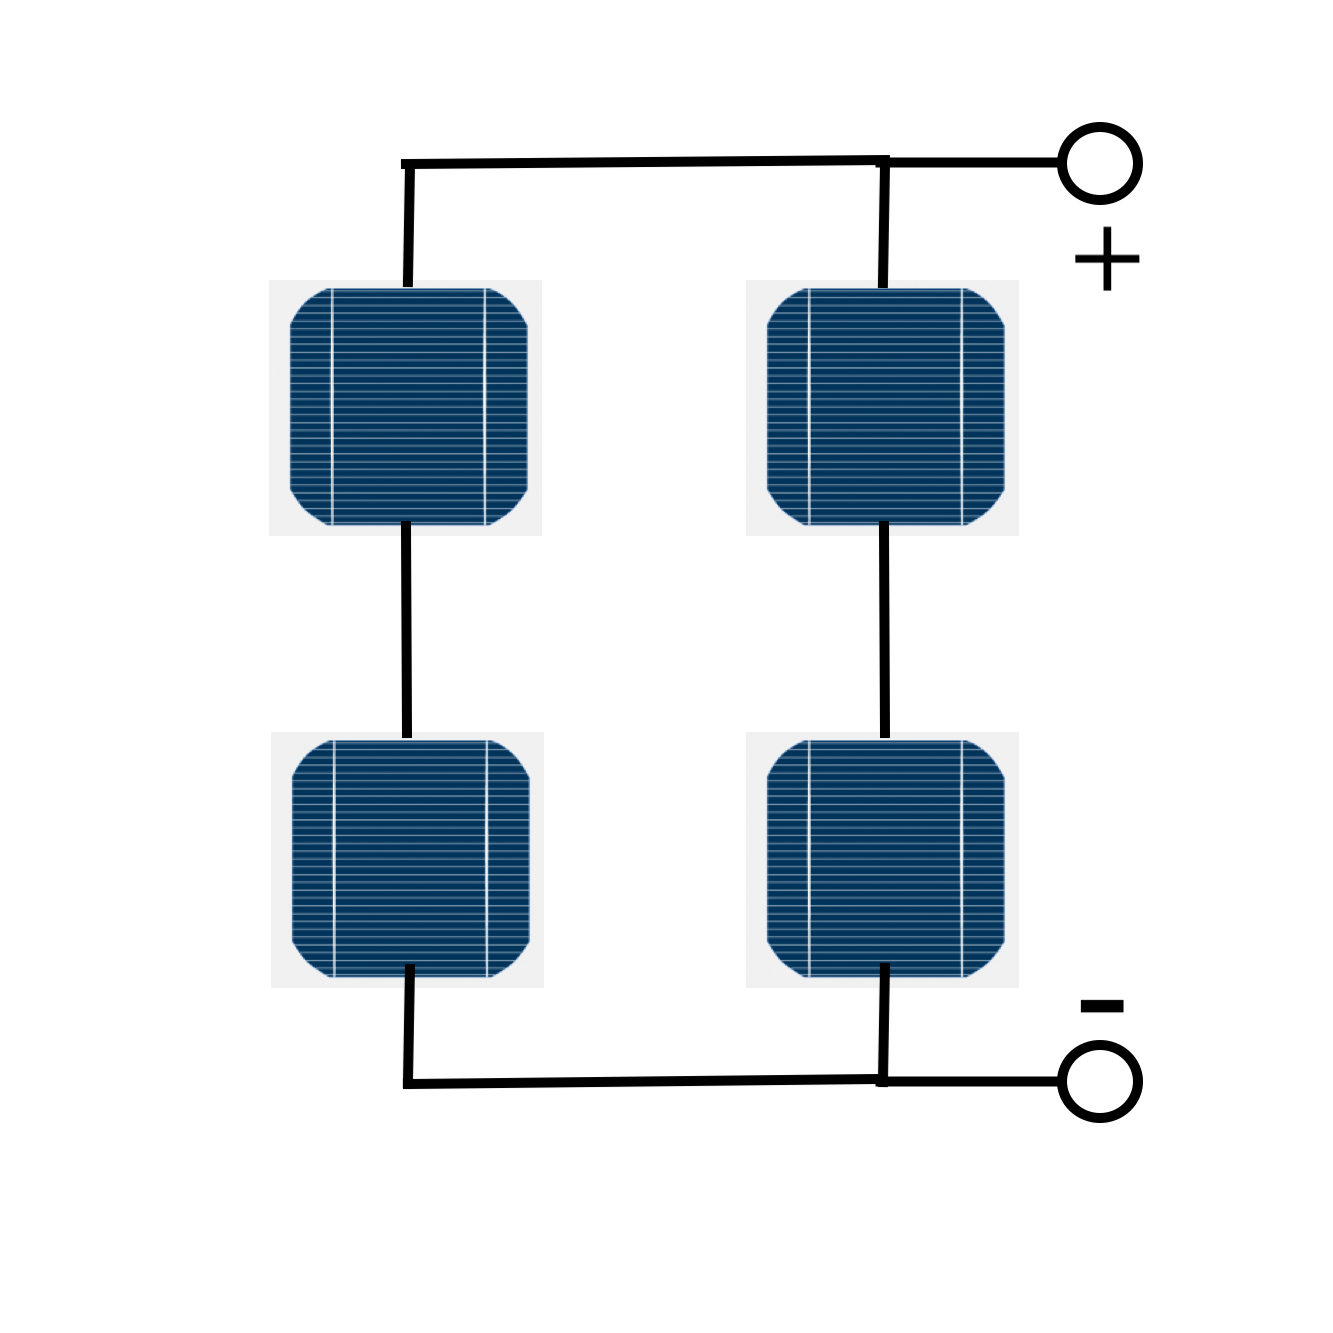
\includegraphics[scale=0.10]{Series-parallel(SP)}
    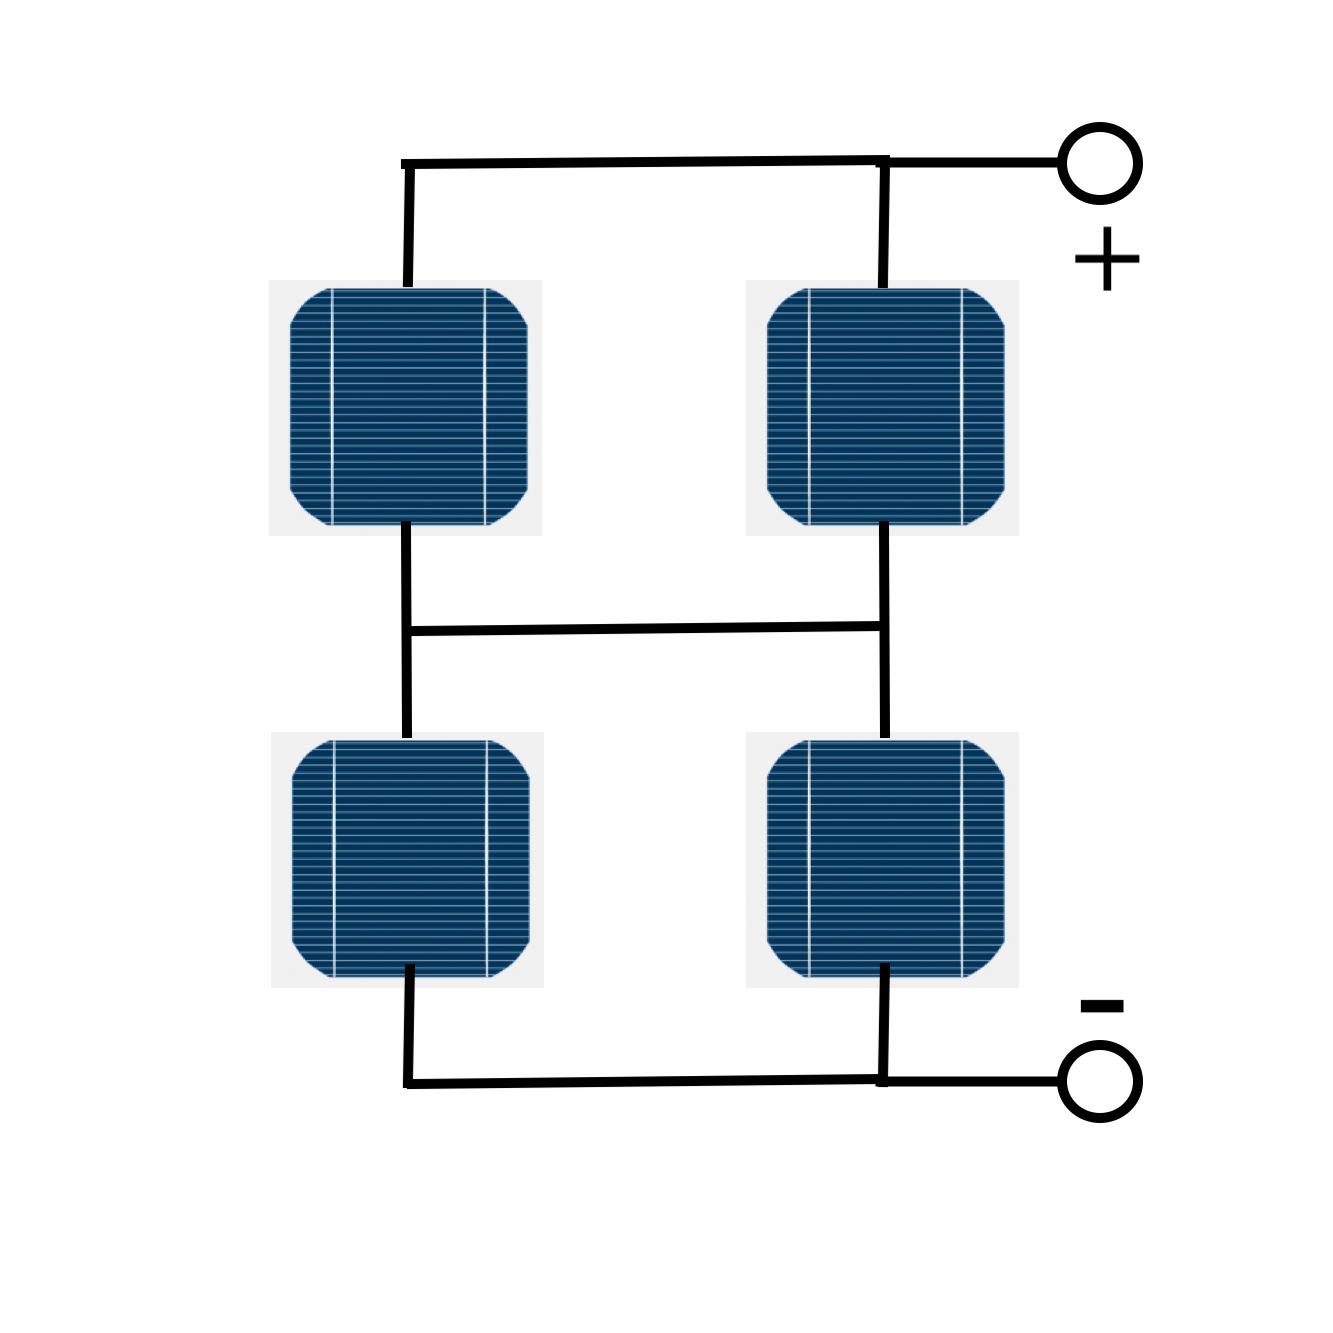
\includegraphics[scale=0.10]{Total-cross-tied(TCT)}
    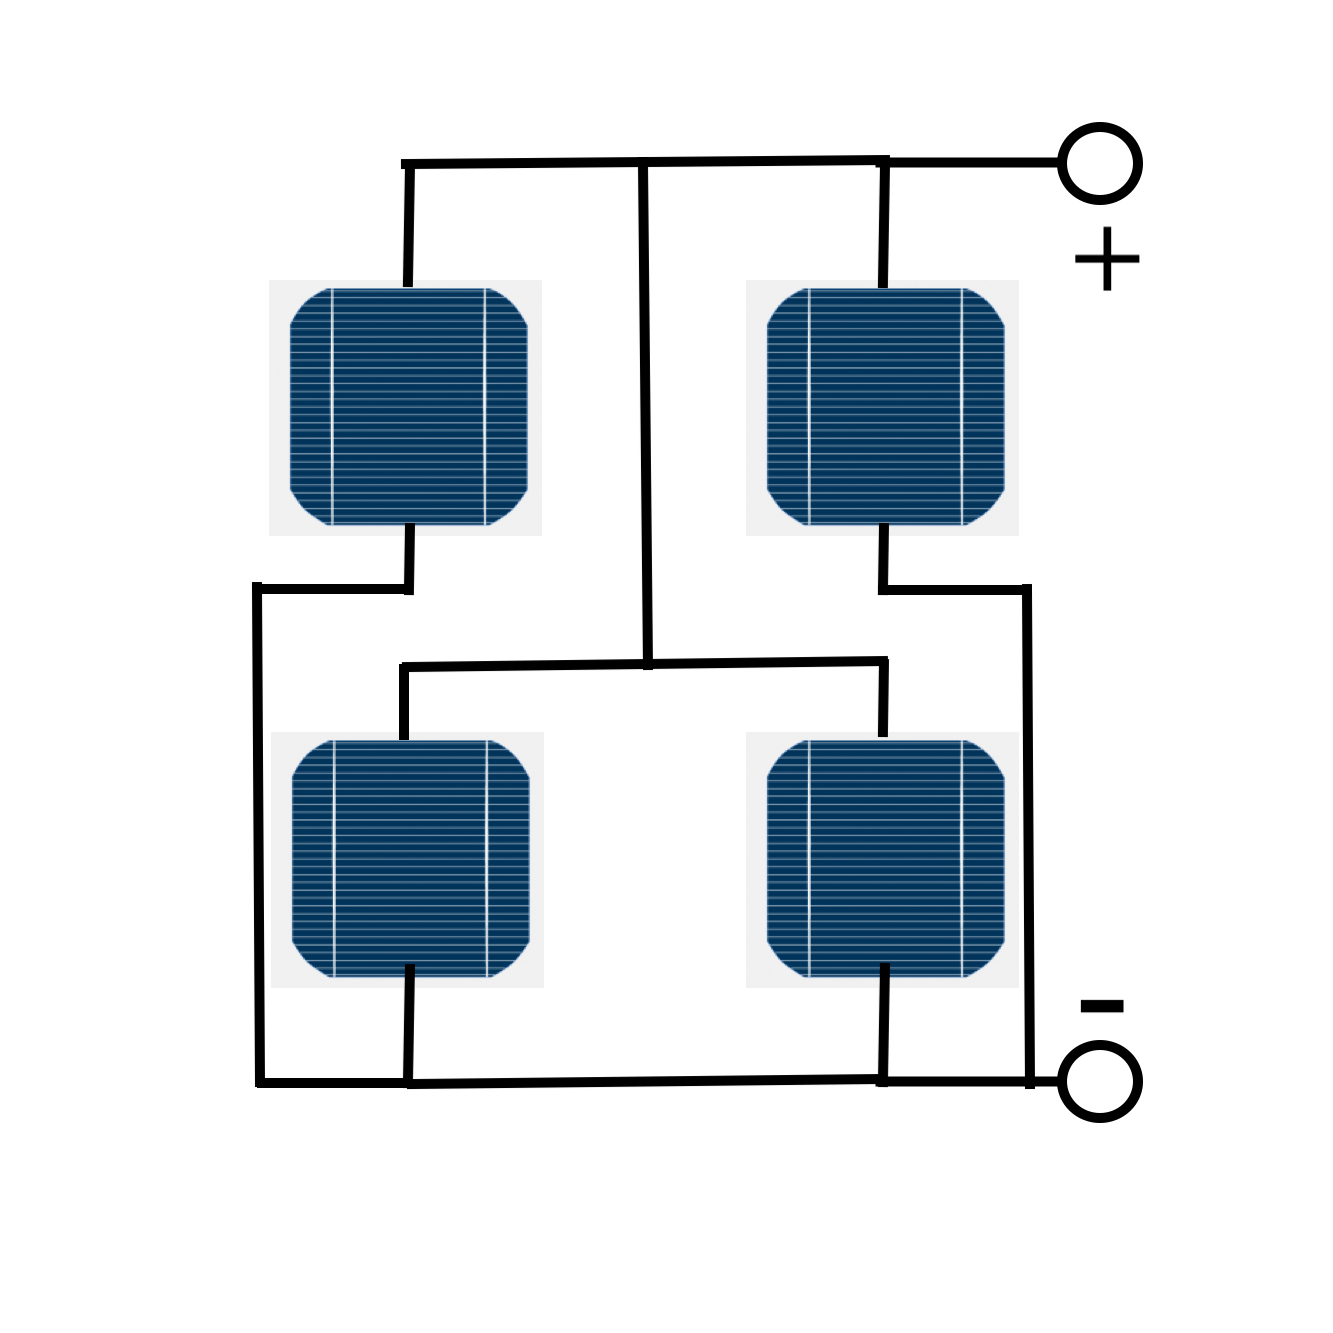
\includegraphics[scale=0.10]{Parallel(P)}
    \caption{From left to right: Series (S), Series-Parallel (SP), Total-Cross-Tied (TCT), Parallel (P)}
    \vspace{-10pt}
    \label{fig:arrayConfigurations}
\end{figure}


However, considering the array voltages it is clear that the only viable arrangement 
is the purely parallel connection. Consider first a pure series connection. In 
section 2.5.1 each PV panel was found to have a max voltage of around 5.5 V. 
The series connection will therefore have a total voltage of about 20+ V. 
The nominal voltage of the series battery pack is \(4 * 3.2 \unit{V} = 12.8 \unit{V} \). 
As the array voltage is higher than the battery voltage, the SMPS must 
be used in the buck configuration. However, the maximum buck input voltage 
is only 7 V\cite{PMOS} and therefore a series connected PV array 
cannot be used. Similarly for the Series-Parallel and Total-Cross-Tied 
arrangements the maximum array voltage will be about 11 V. However, 
as will be discussed in section 2.5.6 the battery pack voltage will 
swing between 10 V and 14.4 V in a charge cycle. The problem is that 
the 11 V array voltage is lower than the highest battery voltage, but
    higher than the lowest battery pack voltage. For the array configuration
to charge the battery pack it would then be necessary to have a power
converter which can both step up and down voltage. Depending on how the 
SMPS is configured it can either function in buck or boost mode, both not 
both at the same time. Thus it is not possible to use either the Series-Parallel
or Total-Cross-Tied configuration. This leaves a purely parallel battery 
pack as the only viable option, which is why it has been chosen. 

\textbf{Maximum Power Point Tracking}
\vspace{10pt} 
\newline
Power provided by PV panels often has to be condition before use. Commonly this 
is done through the use of a two-stage power converter. The first stage of the power
converter does maximum power point tracking to ensure the panels provide as 
much power as possible. The second stage ensures that the power is exported at the
required voltage or current\cite{green}. As the energy submodule only has
access to a single SMPS device it is not possible to implement such a two stage
power converter. Meaning that at any time it will only be possible to either operate 
at the maximum power point or have the power be outputted at the correct current/voltage.
This is however not a problem as the goal of the PV panels is not to output the 
maximum amount of power, but simply to provide the power demanded by the charging algorithm. 
As will be shown in later sections, during charging it is desirable to draw a set
current from the SMPS output. Even if the PV panels could produce more power i.e.
provide a higher current than what is being drawn, it is not desirable to increase 
the output current. As such, the system does not need conventional MPPT. However,
as is discussed below, if the PV panels cannot provide the demanded power some sort 
of power tracking must be implemented. 

\begin{wrapfigure}[18]{r}[0pt]{0.5\textwidth}
    \begin{center}
        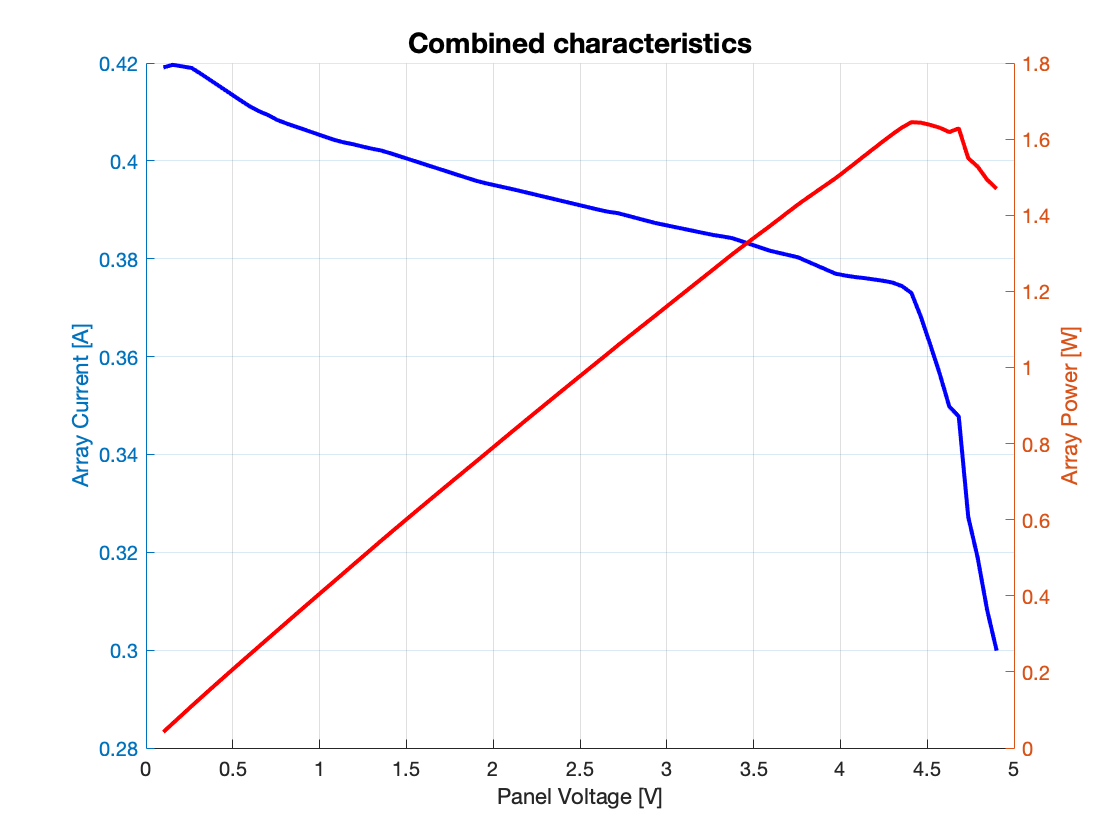
\includegraphics[width=0.48\textwidth]{Combined.png}
    \vspace{-15pt}
    \end{center}
    \caption{IV-curve (blue) and power curve (red) of the parallel configured PV array lit by lamp}
    \label{fig:parallelArray}
\end{wrapfigure}

Consider an SMPS being used to charge a battery pack at a set current. 
If the actual current on the output is lower than the setpoint, one would attempt
to increase the output current by increasing the output voltage. For an SMPS this
is achieved by increasing the duty cycle. Similarly, if the output current is too
high one would attempt to lower the output current by lowering the duty cycle. From 
these considerations we see that increasing and decreasing the duty cycle is 
associated with higher and lower output power respectively. Now compare this with
the IV and power characteristics of the parallel PV array shown in 
Figure ~\ref{fig:parallelArray}. For an SMPS, increasing the duty cycle 
will lower the input resistance, causing the input current to increase. As increasing
the duty cycle increases the output power so too must increased input current lead to
increased input power for an equilibrium to exist. However, increased input current
only gives increased output current if the PV panels are operating in the region to the right of the
maximum power point. Thus this is the region one would want the panels to operate in.

To ensure that the PV panels are operating in the correct region, start with a duty
cycle of 0 and increase it until the output current/voltage is at the desired value.
If the desired operating point requires less power than what the PV array can provide,
then an equilibrium should be found as the duty cycle is increased. If however the 
desired operating point requires more power than the PV panels can provide, then no 
equilibrium can exist and the duty cycle will increase to 1 without ever reaching the
desired operating point. Thus, if the duty cycle ever reaches 1 during operation
the charging algorithm must be trying to draw more power from the SMPS than is 
possible. If so, the charging algorithm must be told to operate a lower power point. How this
is implemented is covered in section ....

\textbf{State of Charge}
\vspace{10pt} 
\newline
The state of charge (SOC) of a battery is defined as the remaining usable charge 
given as a percentage of the battery’s total charge capacity\cite{DICKINSON2009452}. There are many 
methods for  estimating the SOC of a battery, the most common of which rely on 
measurements of the voltage and/or current of the battery\cite{DANKO2019186}. The perhaps 
simplest SOC estimation method is to measure the open circuit voltage (OCV) 
of the battery and then calculate the SOC using a formula or a lookup table. 
For many types of battery this is a good estimation method. An example is 
lead-acid batteries, for which the OCV varies approximately linearly with the 
SOC. However, as was shown figure ~\ref{fig:efficiency}, this is not the case 
for LiFePO4 batteries. For LiFePO4 cells the voltage is nearly constant for 
a majority of each charge/discharge cycle. Any measurement error or change in 
OCV due to current recently flowing through the battery, would therefore produce large 
SOC estimation errors. This holds true for all SOC methods relying purely on 
voltage measurements and they are therefore not good alternatives. 

An alternative SOC estimation method is Coulomb counting, where the current 
flowing through the battery is integrated to find the net charge that has 
left or entered the battery. Seeing as charge is a conserved quantity nearly 
all charge put into the battery will be available during discharge. As such, 
the SOC will vary nearly perfectly linearly with the integrated current. 
The sources of error for Coulomb counting are mainly the Coulombic efficiency 
of the batteries and current measurement errors. However, using correction 
methods the error can be kept small, on the order of 1-2\%\cite{NG20091506}. Given the 
simplicity of the estimation method, this is a very small error. Other 
estimation methods, such as Kalman filters and neural networks, are claimed 
to give higher estimation accuracies\cite{DANKO2019186}. However given the already high 
accuracy of Coulomb counting the improvement is marginal. Moreover, they 
are far more complex both computationally and in implementation. As such, 
Coulomb counting was deemed the best option for SOC estimation.

SOC is a measure of charge and not energy. It is necessary to estimate 
the range of the rover. The obvious way of doing this is to track the 
power consumption and speed of the rover. Dividing the energy left in 
the batteries by the power and multiplying by the speed gives an estimate 
of the range under the current operating conditions. The problem however, 
is that the SOC only gives the usable current and not the usable energy 
left in the battery. As the SOC of the battery decreases, so too does it 
voltage, meaning that at lower states of charge each mAh will provide less 
energy than at higher states of charge. To account for this, during discharging 
the BMS logs the energy output of the battery alongside the SOC. From this data 
it is possible to create a lookup table which relates the current SOC to how 
much energy it is still possible to draw from the battery. This is the method 
which will be used to find the energy left in the battery. 

\textbf{State of Health}
\vspace{10pt} 
\newline
The state of health of a battery is a measure of its current condition and 
performance compared to when it was new\cite{mpower}. Indicators of a battery’s state 
of health include battery charge capacity, energy capacity, cell voltage 
balance, and the number of completed charge/discharge cycles\cite{https://doi.org/10.1002/er.3598}. All these 
indicators are tracked during operation and stored on the SD-card as to 
retain data when the Arduino is not being powered. Over the course of its 
lifetime the SOH of a battery will naturally degrade. However, through SOH 
maintenance the degradation can be slowed significantly. Most importantly 
for a series battery pack is to keep the battery cells balanced, as 
unbalanced battery cells lead to lower capacity and faster cell degradation\cite{texas}. 

To facilitate balancing, each of the provided battery boards have mounted 
resistors which through a MOSFET can be connected to the battery cell. 
Connecting a cell to the resistors on the battery board will lead to a 
small extra current flowing out of the cell, slowly discharging it. 
During operation one must decide when to switch said resistors on and 
off to keep the cells balanced. Usually, balancing is only done towards 
the end of a charge cycle\cite{texas}. There are several reasons for this. Firstly, 
passive balancing requires energy to be expended and will therefore reduce 
the total amount of usable energy in a battery if done during discharging. 
Secondly, differences in impedance and charge curves between cells might 
make it look as though a cell is charged more than others, but the voltage 
difference might disappear naturally as the battery is charged more or as 
charge current is reduced towards the end of a charge cycle. As such, the 
implemented charging algorithm only does balancing during the constant 
voltage part of charging. The balancing is done using the code shown in 
Figure~\ref{fig:balancingCode}. During CV charging it is desirable that all cells have a voltage 
of 3600 mV. If any cell has a voltage which is higher than 3600 mV its 
voltage is too high and the dissipative resistors are switched on to lower 
the voltage to the voltage set point. 

\begin{figure}[H]
    \centering
    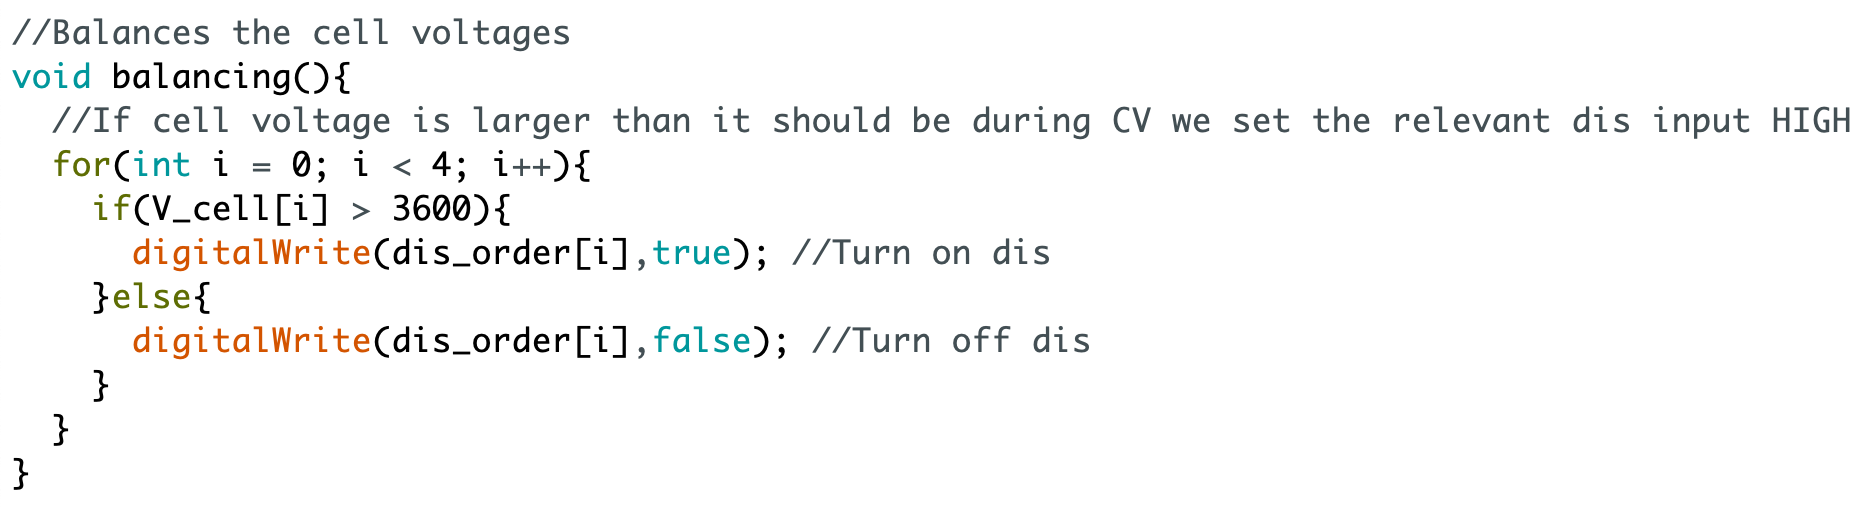
\includegraphics[width = \textwidth]{Balancing_code.png}
    \caption{Function called while charging at high SOC to balance out the voltage of the cells.}
    \vspace{-10pt}
    \label{fig:balancingCode}
\end{figure}

Alongside the constant voltage charging algorithm this code was extremely 
successful at balancing the cells. The balancing is shown in action in Figure~\ref{fig:balancing}. 
One by one, the cell voltages are brought up to and kept at 3600 mV. Even with 
an initial voltage difference of 200 mV, balancing only takes about 
1000 seconds = 17 minutes. 


\begin{figure}[H]
    \centering
    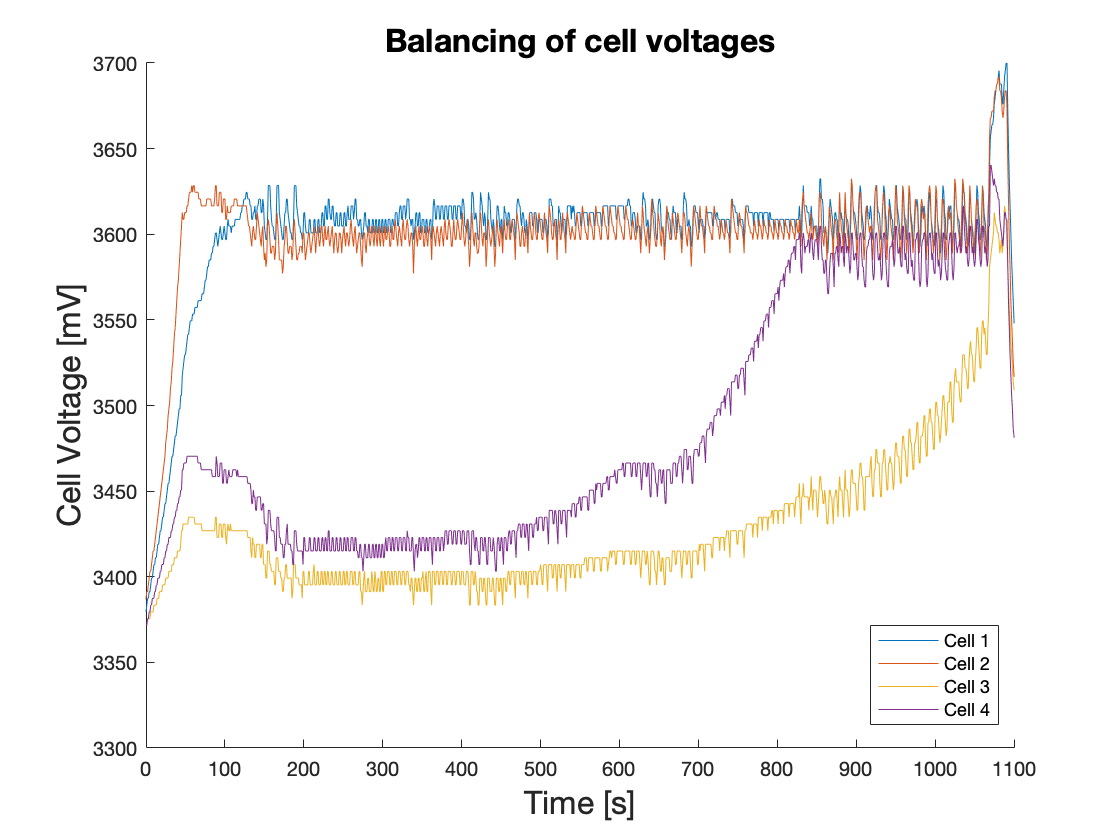
\includegraphics[width=0.48\textwidth]{balancing.png}
    \caption{Cell voltages as they are being balanced, ignore voltage spikes at end as they are not related to the balancing.}
    \label{fig:balancing}
\end{figure}

\textbf{Communicating with Other Modules}
\vspace{10pt} 
\newline
Though it is not necessary to fully integrate the energy module with the rest of 
the rover, other submodules, specifically command, needs access data such as the 
battery SOH and SOC. For communicating with other modules the Arduino shield has 
a set of UART ports. However, as group members were not in the same location it 
was not possible to physically connect the energy module to the rover, which is 
necessary to use UART. As such, an alternative approach was employed. First the 
Arduino was connected to a computer via USB. On the computer a Python script was 
run [8]. At the start the Python script establishes a connection to a server 
created by running a similar script on the command module [9]. After a 
connection has been established the Python script starts reading the serial data 
coming from the Arduino and transmits it using TCP to the command module. Each 
message coming from the Arduino is in CSV form where the first entry is the 
message ID, which allows the command script to decode what type of data is being 
sent. What data do we send? 

\textbf{Physical Integration of the Energy Module}
\vspace{10pt} 
\newline
Due to students being in different locations the energy module will not be physically 
integrated with the full rover. However, outlined below is one way the energy module 
could be physically connected if necessary. 

The energy module can either be integrated as a charging station or, as is more 
common for mars rovers, be mounted directly on the rover itself. The advantage of 
implementing it as a charging station is that one would only ever charge or discharge 
the battery at a given time. This makes it easier to track the current and power 
in and out of the system and create charging/discharging algorithms. There are 
two major drawbacks to using charging station. Firstly, the rover would get a 
severely reduced range as it always needs to be able to make it back to the 
charging station before its battery is depleted. Secondly, if the rover is detached 
from the charging station, how will the energy module be able to track the cell 
voltages and SOC. It might be possible to create a system where different 
microcontrollers keep track of energy when the rover is connected and when it 
is not connected to the charging station. However, a likely simpler solution 
is to mount the energy module on the rover. A mounted system will increase 
the range, but requires the ability to charge and discharge the battery at the same time.

Assuming that a mounted solution is used there are two main design problems 
to be solved. Firstly, how will power be supplied to each of the rover components 
and secondly, how is simultaneous charging and discharging facilitated?

As shown in Figure ? the rover has 4 separate voltage regions. The battery and 
PV array have already been discussed. The new regions are the 5V node used to power 
the FPGA and micro-controllers, and the variable voltage node used to power the 
motors. Currently, the 5V used to power the control circuitry is also used to power 
the drive SMPS. The most straight forward way to connect the energy sub-module to 
the rest of the rover would therefore be to step down the battery voltage to 5V 
using a buck SMPS and connect the SMPS output where the battery pack is currently 
connected. However, this is very energy inefficient as the power for the motor needs 
to pass through two SMPS devices before being used, potentially leading to high power 
losses. A better way of connecting the energy module would involve separating the 
drive SMPS from the 5V node. Instead the drive SMPS could be directly connected to 
the battery. Then another SMPS or linear voltage regulator would be connected to the 
battery to create 5V power for the control circuitry. A sketch diagram of the 
connections is shown in Figure ?. One problem exists however with this solution: 
The 10.0 – 14.4 V of the battery is higher than the SMPS maximum input voltage. 
A way to solve this would be to exchange the PMOS on the SMPS board for another NMOS, 
which would increase the maximum input voltage.

In this design there are three systems through which current either flows in or 
out of the battery. To keep track of the SOC and ensure that the batteries are 
being charged or discharged at an appropriate it is therefore necessary to collect
current data for all the power converters. This data could be relayed through control 
and read in on the energy Arduino through UART. The net battery current can then be 
calculated by simply adding together the current passing through each of the power 
converters. The rest of the charge algorithm would not be affected by this. This 
implementation also integrates well with the integrated power point tracking algorithm 
and will make sure that the demanded charge current is not higher than what can be 
provided while simultaneously powering the rover.

%End of energy functional section

%End of funtional section

\section{Implementation}

\subsection{Vision}

\subsection{Control}

\subsection{Command}

\subsection{Drive}

\begin{center}
\textbf{Abstract}
\end{center}
The purpose of the driving module is to make an accurate movable rover that can 
move forward, backward, rotate clockwise and anticlockwise at the desired speed.
Also, to process coordinates and send them back to the control module in order 
the rover to map the area.

\textbf{General Specifications}

Initially, the main goal of the driving subsystem was to make a movable rover. 
The specifications and the limitations of the SMPS, Arduino and the DC motors, 
needed to be known.  The first challenge was to find a way to measure the 
rotations per minute (RPM) of the DC motors, precisely. The solution was to 
stick a small piece of paper on the rotating axes of the DC motor. Additionally,
one screwdriver was placed perpendicularly to the small piece of paper. This was
done because each time the DC motor completed one whole rotation the small piece
of paper would ``trigger'' the screwdriver and generate a distinctive sound.
Finally, the only unsolved part was how to pick up that sound. So, the 
microphone of one set of earphones was placed close enough to the DC motor in order 
to pick up that distinctive sound. Then, the whole process was recorded, leading 
to the following outstanding outcome. The recorded sound was processed with an 
audio application and every time the DC motor completed a whole period the 
waveform of the recorded sound had a spike with a recognisable magnitude. 
Finally, the time difference between one spike to the following one was the 
period (T) of the DC motor. 
Then only the conversion from time to RPM was left and in order to find the RPM,
the following formula was used: \( RPM=\frac{60}{T} \) 

%%%%%%%%%%%%%%%%%%%% Figure/Image No: 1 starts here %%%%%%%%%%%%%%%%%%%%

\begin{figure}[H]
\begin{Center}
\advance\leftskip 0.23in		
    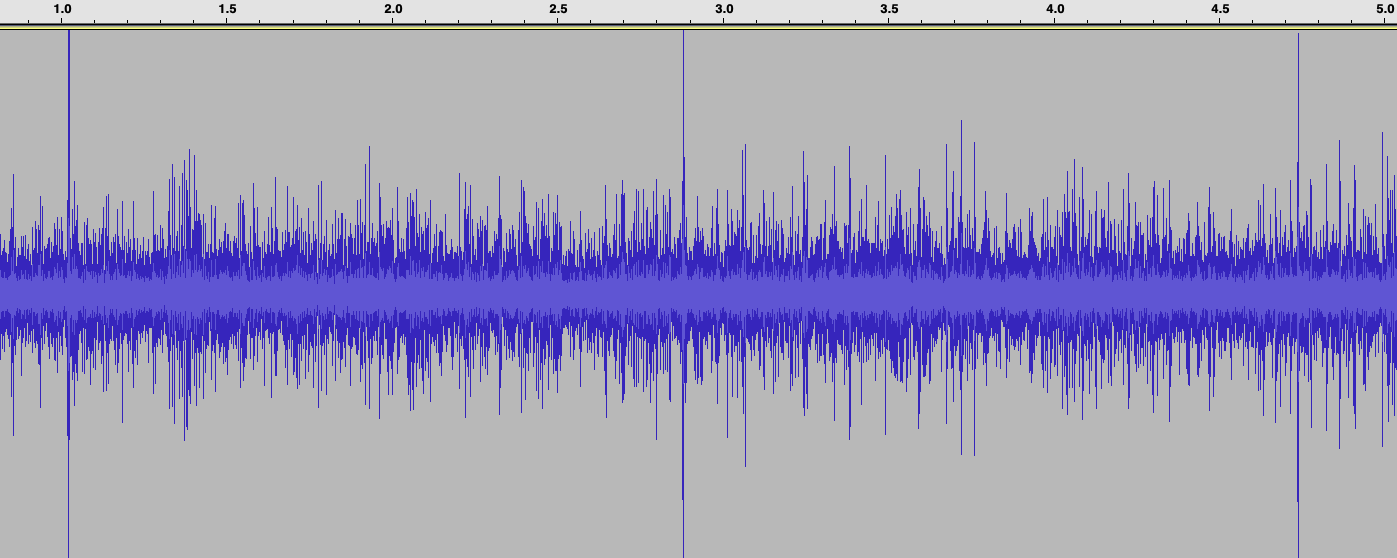
\includegraphics[width=5.06in,height=2.02in]{./media/image2.png}
	\caption{Shows the spikes that correspond to a period(T)}
		\label{Shows the spikes that correspond to a period(T)}
\end{Center}
\end{figure}


%%%%%%%%%%%%%%%%%%%% Figure/Image No: 1 Ends here %%%%%%%%%%%%%%%%%%%%




%%%%%%%%%%%%%%%%%%%% Figure/Image No: 2 starts here %%%%%%%%%%%%%%%%%%%%

\begin{figure}[H]
	\begin{Center}
		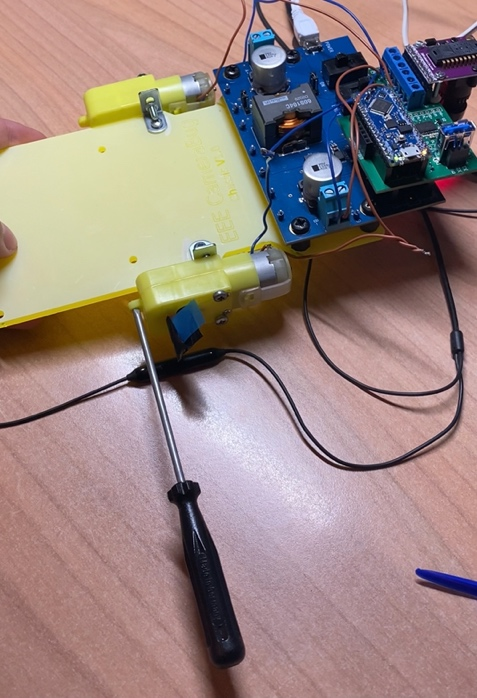
\includegraphics[width=2.16in,height=3.15in]{./media/image1.jpeg}
		\caption{During the recording process}
		\label{figDuring_the_process_of_recording}
	\end{Center}
\end{figure}


%%%%%%%%%%%%%%%%%%%% Figure/Image No: 2 Ends here %%%%%%%%%%%%%%%%%%%%

In the following table some basic specifications have been measured:


%%%%%%%%%%%%%%%%%%%% Table No: 1 starts here %%%%%%%%%%%%%%%%%%%%


\begin{table}[H]
 			\centering
\begin{tabular}{p{2.93in}p{2.93in}}
\hline
%row no:1
\multicolumn{1}{|p{2.93in}}{\Centering \textbf{\textit{Input}}} & 
\multicolumn{1}{|p{2.93in}|}{\Centering \textbf{\textit{Output}}} \\
\hhline{--}
%row no:2
\multicolumn{1}{|p{2.93in}}{Voltage $ \approx $ 5V} & 
\multicolumn{1}{|p{2.93in}|}{Minimum Operating Voltage: 1.384V \par Maximum Arduino's Voltage for accurate conversion: 4.096V \par } \\
\hhline{--}
%row no:3
\multicolumn{1}{|p{2.93in}}{Minimum Current: 0.134A \par Maximum Current: 0.22A \par } & 
\multicolumn{1}{|p{2.93in}|}{Minimum Operating Current: 0.035A \par Maximum Arduino's Current for accurate conversion: 0.060A \par } \\
\hhline{--}

\end{tabular}
 \end{table}


%%%%%%%%%%%%%%%%%%%% Table No: 1 ends here %%%%%%%%%%%%%%%%%%%%

\textbf{Speed Levels}

One of the main goals was to make the user interface with the rover relatively 
simple and that is why the idea of introducing 5 speed levels came up. 
Specifically, the idea behind those 5 speed levels, is to avoid using km/h or 
mph because the range of km/h is really small (0.17km/h-0.62km/h) and the range 
for the mph is even smaller (0.11mph-0.38mph) so, it will confuse the user. Thus,
one way to simplify the speed range is to set 5 speed levels that can be 
understood easily and be user friendly as well. Additionally, it is more 
convenient and straightforward as it does not require further knowledge 
(voltages, RPM).

In order to find the true range of voltages the rover's limits needs to be found. 
The code that is responsible for the voltage range has a reference voltage of 
4.096V. The value 4.096, is the Arduino's upper threshold for accurate 
conversion. On the other hand, the buck SMPS can generate up to 4.8V 
( due to the power losses it cannot generate exactly 5V). If the Arduino's 
reference voltage is increased then if, for example, a 2.5V reference voltage 
is sent to the rover, it  would not ``generate'' 2.5V as an input for the 
DC motors. This happens because the Arduino can handle only up to 4.096V and 
if this value is exceeded then the conversion will not be accurate. On the other 
hand, the lower limit is 1.46V because everything beyond that will not have enough 
power to move the rover. To conclude, the voltage range is from 1.46V to 4.096V in 
order to have a movable and an accurate rover. So, that is why the speed levels 
are divided like that. Those 5 speed levels can easily be ``corresponded'' to a 
specific voltage, and a specific voltage can easily be ``corresponded'' to a 
specific velocity.  After the the RPMs were found then, they were converted to 
speed values by the following formula:

$$ v \left(\frac{km}{hr}\right) = r \times \frac{2\pi}{60} \times N \left( rpm \right) \times 3.6  $$
% \[  \]  \[ v \left( \frac{km}{h} \right) =r\ast\frac{2 \pi }{60}\astN \sleft( rpm \right) \ast3.6 \] 
where r is the radius of the wheel and is equal to 3.4cm and the number 3.6 is used to convert m/s to km/h. 



%%%%%%%%%%%%%%%%%%%% Table No: 2 starts here %%%%%%%%%%%%%%%%%%%%


\begin{table}[H]
 			\centering
\begin{tabular}{p{0.67in}p{0.57in}p{0.62in}p{0.58in}p{0.78in}p{0.47in}p{0.47in}p{0.5in}}
\hline
%row no:1 
\multicolumn{1}{|p{0.67in}}{Speed Level} & 
\multicolumn{1}{|p{0.57in}}{RPM} & 
\multicolumn{1}{|p{0.62in}}{km/h} & 
\multicolumn{1}{|p{0.58in}}{mph} & 
\multicolumn{1}{|p{0.78in}}{Output Voltage(v)} & 
\multicolumn{1}{|p{0.47in}}{Input Voltage (V)} & 
\multicolumn{1}{|p{0.47in}}{Input Current (A)} & 
\multicolumn{1}{|p{0.5in}|}{Pin(W)} \\
\hhline{--------}
%row no:2
\multicolumn{1}{|p{0.67in}}{\textbf{Very fast }} & 
\multicolumn{1}{|p{0.57in}}{48.58 } & 
\multicolumn{1}{|p{0.62in}}{0.6227 } & 
\multicolumn{1}{|p{0.58in}}{0.3869 } & 
\multicolumn{1}{|p{0.78in}}{4.05} & 
\multicolumn{1}{|p{0.47in}}{4.95} & 
\multicolumn{1}{|p{0.47in}}{0.216} & 
\multicolumn{1}{|p{0.5in}|}{1.0692} \\
\hhline{--------}
%row no:3
\multicolumn{1}{|p{0.67in}}{\textbf{Fast}} & 
\multicolumn{1}{|p{0.57in}}{41.27 } & 
\multicolumn{1}{|p{0.62in}}{0.5289 } & 
\multicolumn{1}{|p{0.58in}}{0.3287 } & 
\multicolumn{1}{|p{0.78in}}{3.4} & 
\multicolumn{1}{|p{0.47in}}{4.96} & 
\multicolumn{1}{|p{0.47in}}{0.192} & 
\multicolumn{1}{|p{0.5in}|}{0.95232} \\
\hhline{--------}
%row no:4
\multicolumn{1}{|p{0.67in}}{\textbf{Regular}} & 
\multicolumn{1}{|p{0.57in}}{32.38 } & 
\multicolumn{1}{|p{0.62in}}{0.4150 } & 
\multicolumn{1}{|p{0.58in}}{0.2579 } & 
\multicolumn{1}{|p{0.78in}}{2.75} & 
\multicolumn{1}{|p{0.47in}}{4.97} & 
\multicolumn{1}{|p{0.47in}}{0.162} & 
\multicolumn{1}{|p{0.5in}|}{0.80514} \\
\hhline{--------}
%row no:5
\multicolumn{1}{|p{0.67in}}{\textbf{Slow}} & 
\multicolumn{1}{|p{0.57in}}{23.92 } & 
\multicolumn{1}{|p{0.62in}}{0.3066 } & 
\multicolumn{1}{|p{0.58in}}{0.1905 } & 
\multicolumn{1}{|p{0.78in}}{2.1} & 
\multicolumn{1}{|p{0.47in}}{4.98} & 
\multicolumn{1}{|p{0.47in}}{0.152} & 
\multicolumn{1}{|p{0.5in}|}{0.75696} \\
\hhline{--------}
%row no:6
\multicolumn{1}{|p{0.67in}}{\textbf{Very Slow}} & 
\multicolumn{1}{|p{0.57in}}{13.89 } & 
\multicolumn{1}{|p{0.62in}}{0.1780 } & 
\multicolumn{1}{|p{0.58in}}{0.1106 } & 
\multicolumn{1}{|p{0.78in}}{1.46} & 
\multicolumn{1}{|p{0.47in}}{4.99} & 
\multicolumn{1}{|p{0.47in}}{0.134} & 
\multicolumn{1}{|p{0.5in}|}{0.66866} \\
\hhline{--------}

\end{tabular}
 \end{table}


%%%%%%%%%%%%%%%%%%%% Table No: 2 ends here %%%%%%%%%%%%%%%%%%%%



One interesting observation is that the relationship between the voltage and the 
RPM is almost linear. This is confirmed in Figure \ref{graph: Output Voltage vs RPM}


 %%%%%%%%%%%%%%%%%%%  %  iGraph 1%%%%%%%%%%%%%%%%%%%%%%

 \begin{figure}[H]
    \centering
    \begin{minipage}{.3\textwidth}
      \centering
      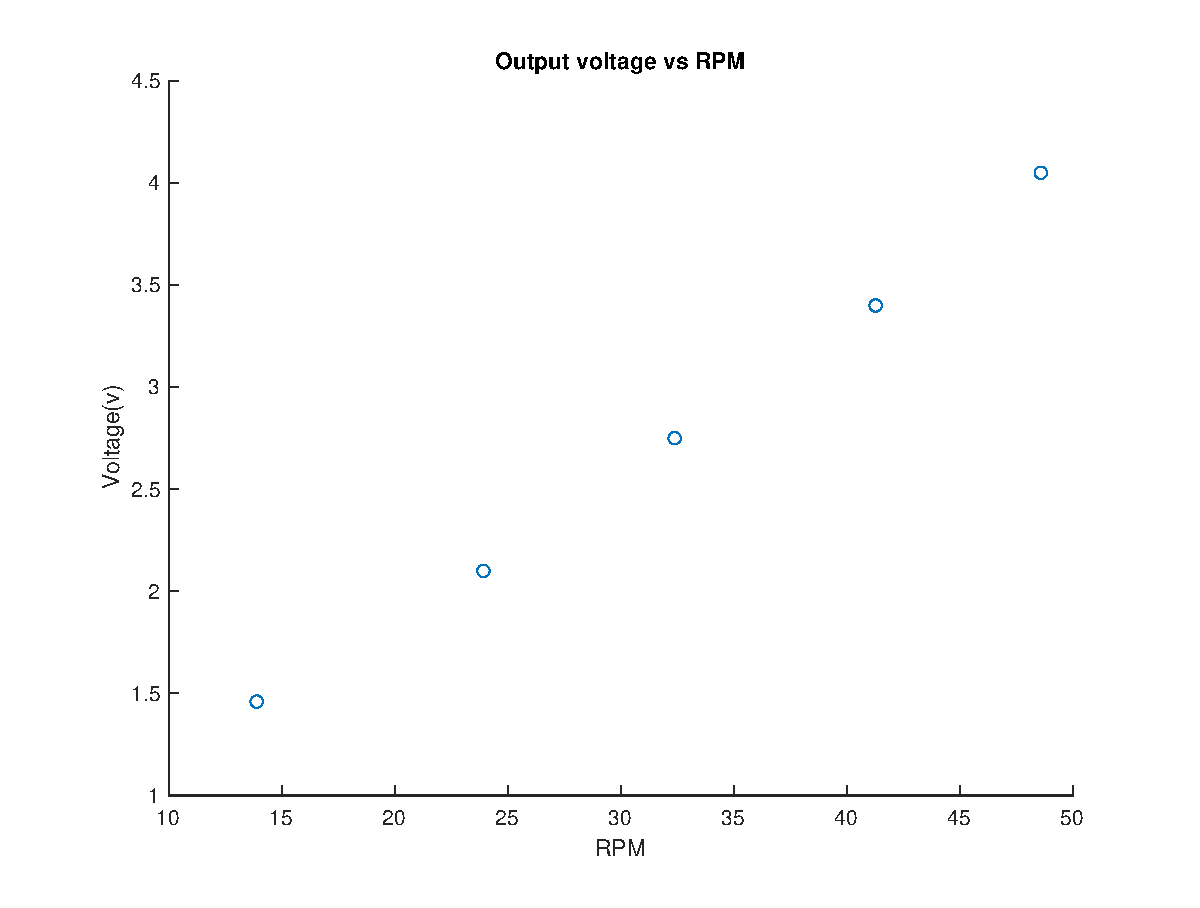
\includegraphics[scale=0.22]{./media/voltagevsrpm.eps}
   \caption{Output Voltage vs RPM}
   \label{graph: Output Voltage vs RPM}
    \end{minipage}%
    %\begin{minipage}{.7\textwidth}
      %\centering
      %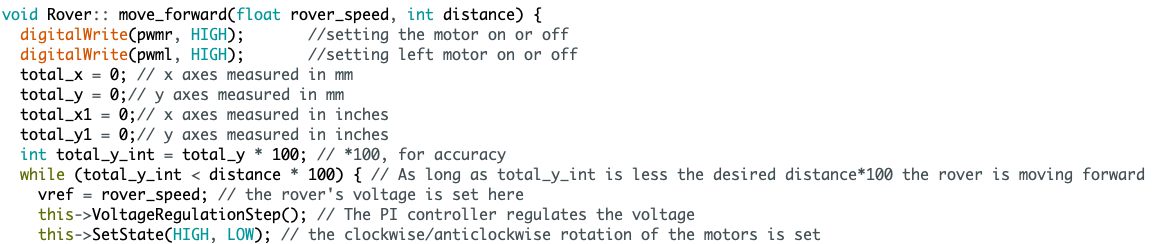
\includegraphics[scale=0.25]{./media/forward.png}
		%\caption{Forward Command Code}
      %\label{fig:Forward Command Code}
    %\end{minipage}
\end{figure}

%\begin{figure}
 %  \centering
  % 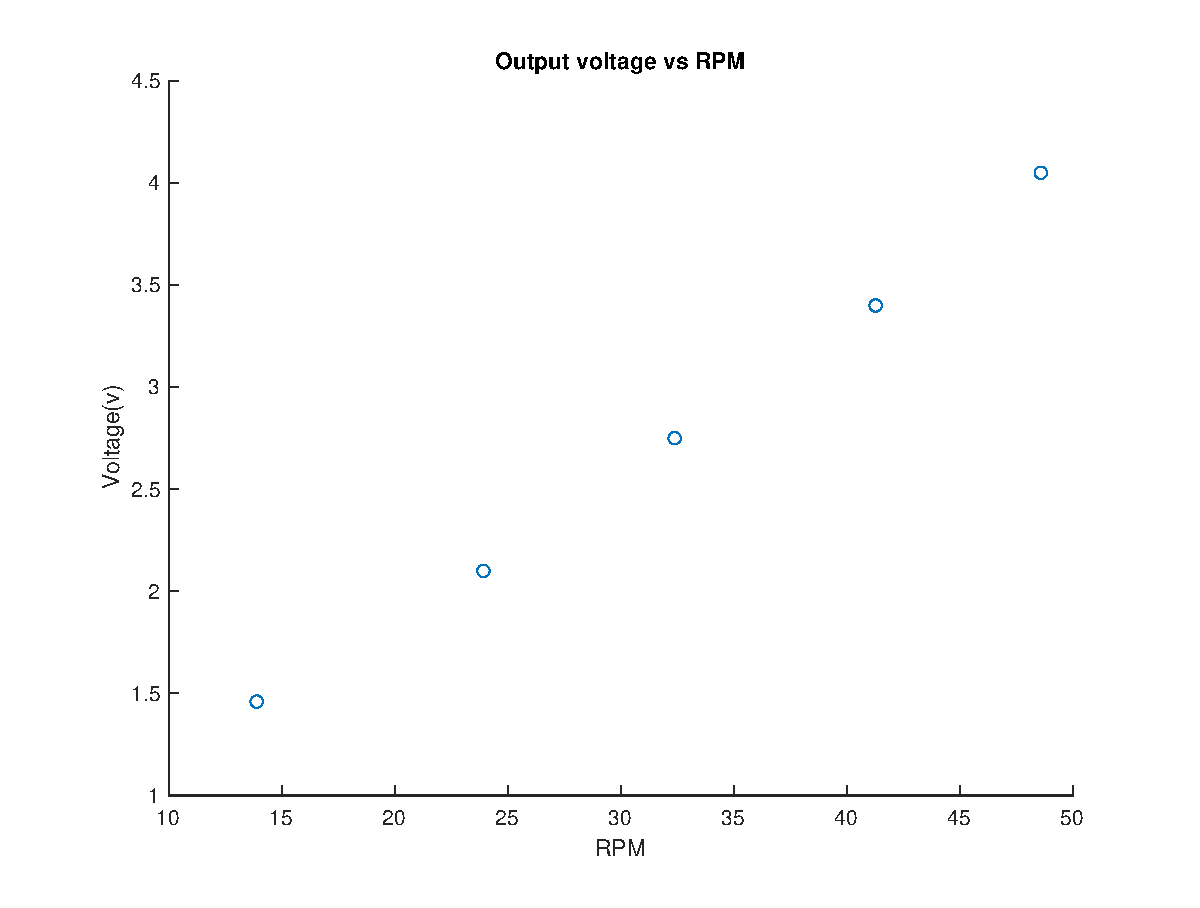
\includegraphics[scale=0.5]{./media/voltagevsrpm.eps}
   %\caption{Output Voltage vs RPM}
   %\label{graph: Output Voltage vs RPM}
%\end{figure}



%%%%%%%%%%%%%%%%Graph2 ends here%%%%%%%%%%%%%%%%%%%%%%%%
\paragraph*{Commands}


After finding the specifications the next step was to make a movable rover. 
Initially, one crucial task to do was to simplify and ``connect''  the two 
sample codes. To do that, there was a need for the use of an object oriented 
approach which would make it feasible to combine functions of the two sample 
codes into two different objects. In this case classes were used to implement 
a rover object and an optical flow sensor object. This allows to use the 
complicated code of the optical flow sensor in a simple way inside the rover 
functions.After, making the code simple and creating classes that would make 
the testing straightforward, 2 major changes were made to the code. Firstly, 
even though the control knob was really helpful to measure some key data, 
for the project it was needed to be able to set output voltages independently 
of the control knob and that is why it was not used. Specifically, the voltage 
of the DC motors is now being controlled by the user with those 5 speed levels. 
Secondly, the optical flow sensor was connected directly to the code that is 
responsible for the movement of the rover. In other words, the rover was able 
to move backward and forward by just setting inside a while loop the desired 
distance and comparing it with the measurements of the optical flow sensor. 
For example, the desired distance is 20cm, the rover will be moving forward 
or backward until the measurements read from the optical flow sensor for the 
y axes are approximately equal to 20cm.

\begin{figure}[H]
	\begin{Center}
		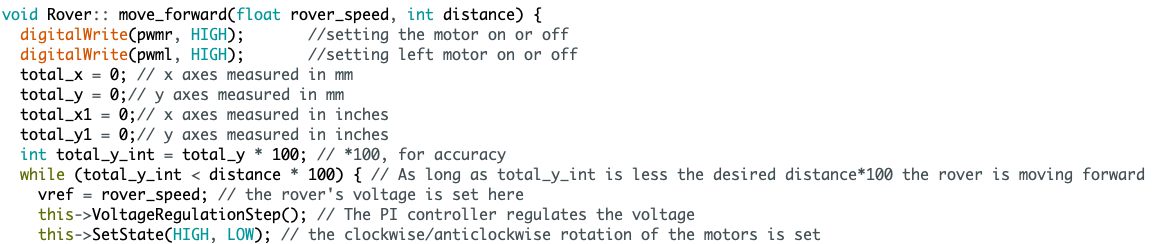
\includegraphics[scale=0.3]{./media/forward.png}
		\caption{Forward Command Code}
	\end{Center}
\end{figure}


Additionally, to make the rover rotate clockwise and anticlockwise the 
following process was implemented: Assuming that the centre of the rover 
(the centre of the imaginary axes that connects the two DC motors) is not 
rotating and it remains in the same position while the main body is rotating, 
then it can concluded that the rover is tracing an arc. The imaginary arc with 
the body of the rover is forming a circular sector. The radius of the imaginary 
circular sector is the length from the centre of the optical flow sensor to the 
centre of the imaginary axes that connects the DC motors. The mathematical 
formula is given as follows  \( \textbf{arc length}= \theta r \), where  \(\theta\)   is 
the angle in radians and \(r\) is the radius. So, to implement this, as seen in Figure \ref{fig: Clockwise Command Code} a while loop 
in the code was implemented to make the rover to rotate as long as the traced 
path of the optical flow sensor is less than the arc length needed to be traced 
to cover a specific angle. For example, if the desired angle is 90\degree \   
or  \( \frac{ \pi }{2} \)  the rover will be rotating until the measured path 
of the optical flow sensor (the x value that is being measured from the optical 
flow sensor) is equal to the angle times the radius. The radius is approximately 
168 mm but in the code it has been adjusted in order the rotation command to be 
accurate.

%\begin{figure}[H]
	%\begin{Center}
		%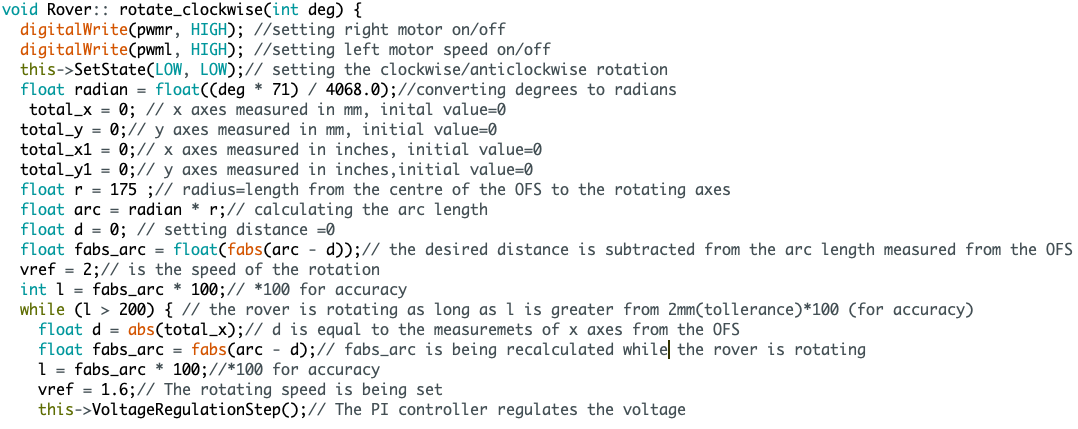
\includegraphics[scale=0.3]{./media/clockwise.png}
		%\caption{Clockwise Command Code}
	%\end{Center}
%\end{figure}

\begin{figure}[H]
    \centering
    \begin{minipage}{.7\textwidth}
      \centering
      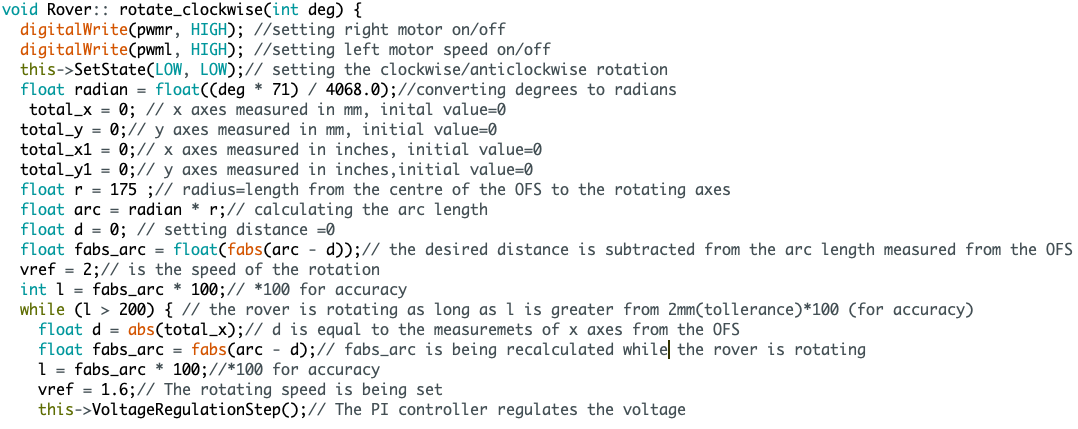
\includegraphics[scale=0.3]{./media/clockwise.png}
      \caption{Clockwise Command Code}
      \label{fig: Clockwise Command Code}
    \end{minipage}%
%%%%%%%%%%%%%%%%%%%% Figure/Image No: 3 starts here %%%%%%%%%%%%%%%%%%%%
    \begin{minipage}{.3\textwidth}
      \centering
      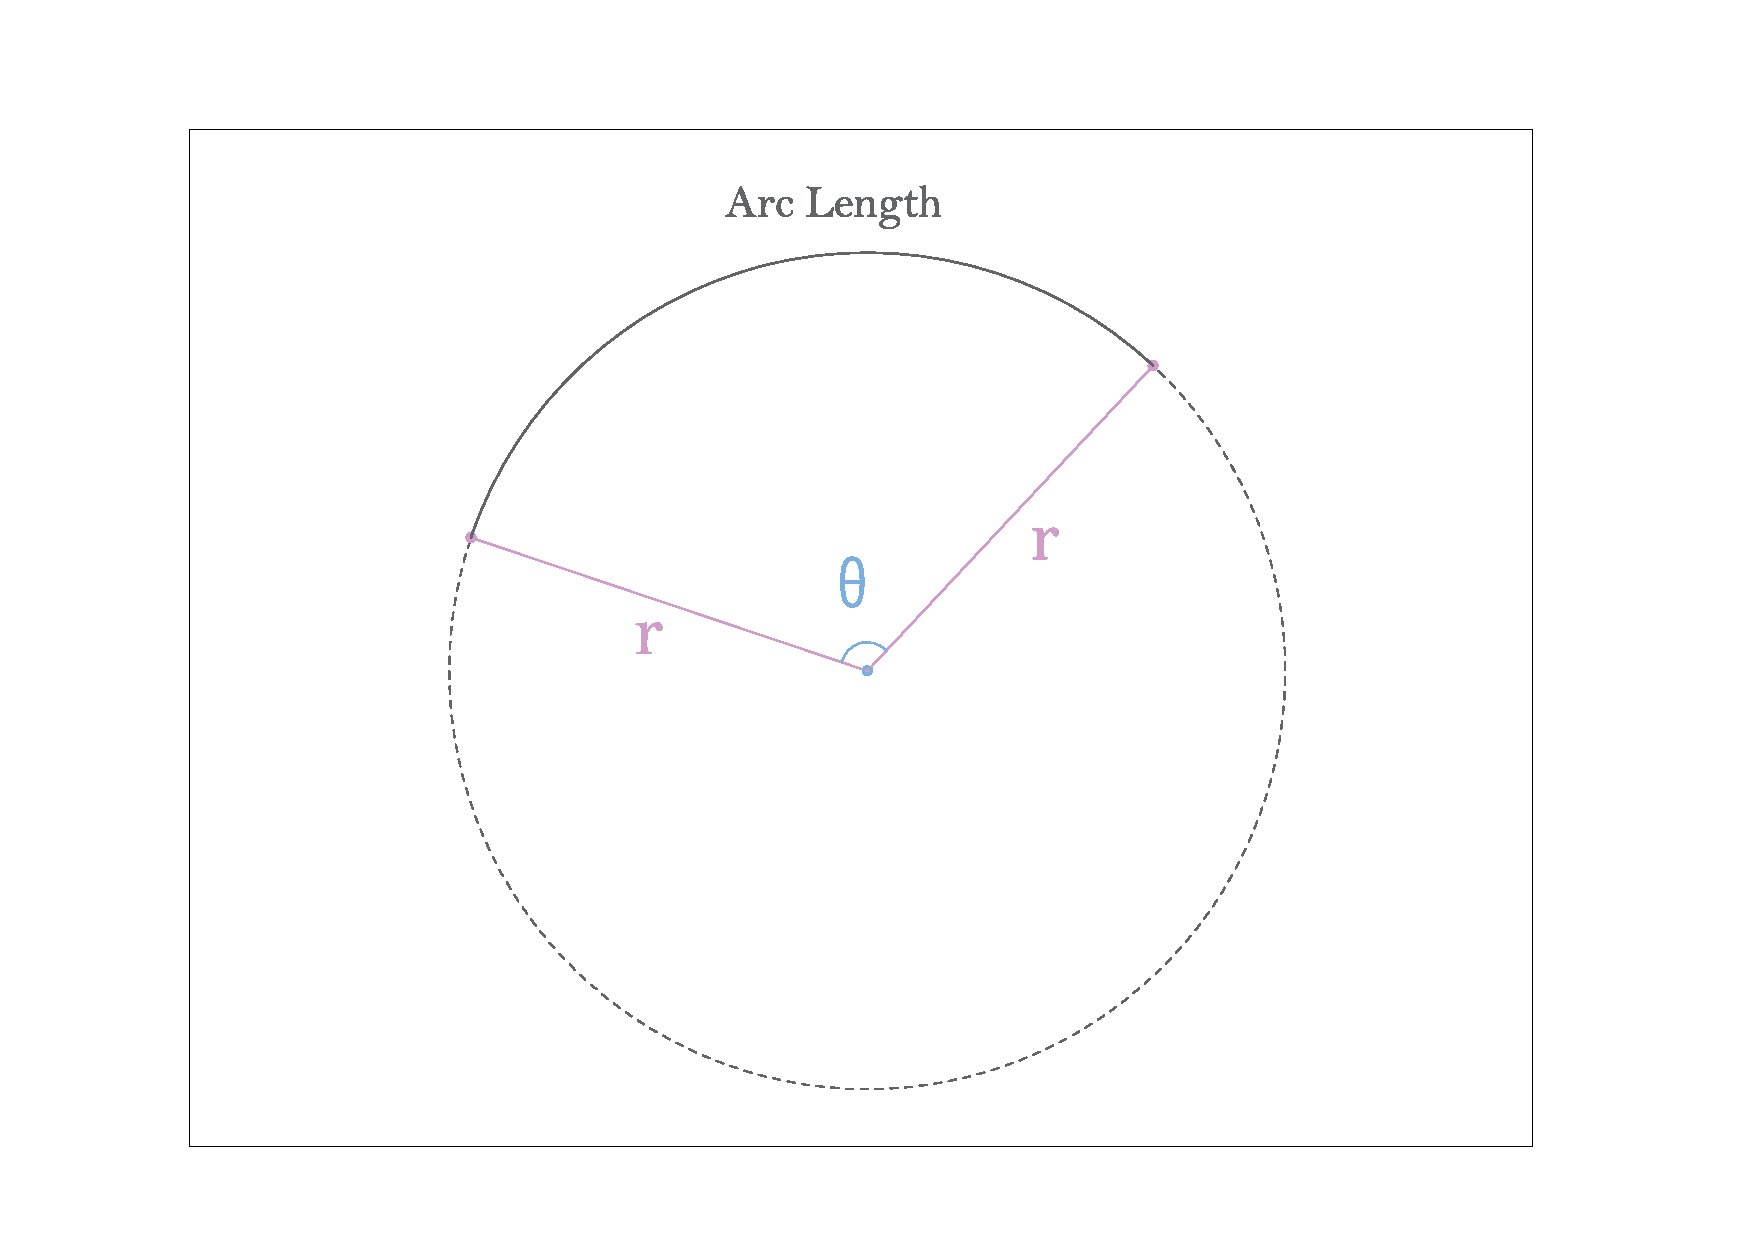
\includegraphics[scale = 0.2]{./media/image3.pdf}
      \caption{The arc that the \\ optical flow sensor is tracing}
      \label{fig: Optical Flow Sensor Arc}
    \end{minipage}
\end{figure}

   
%\begin{figure}[H]
%\begin{center}
%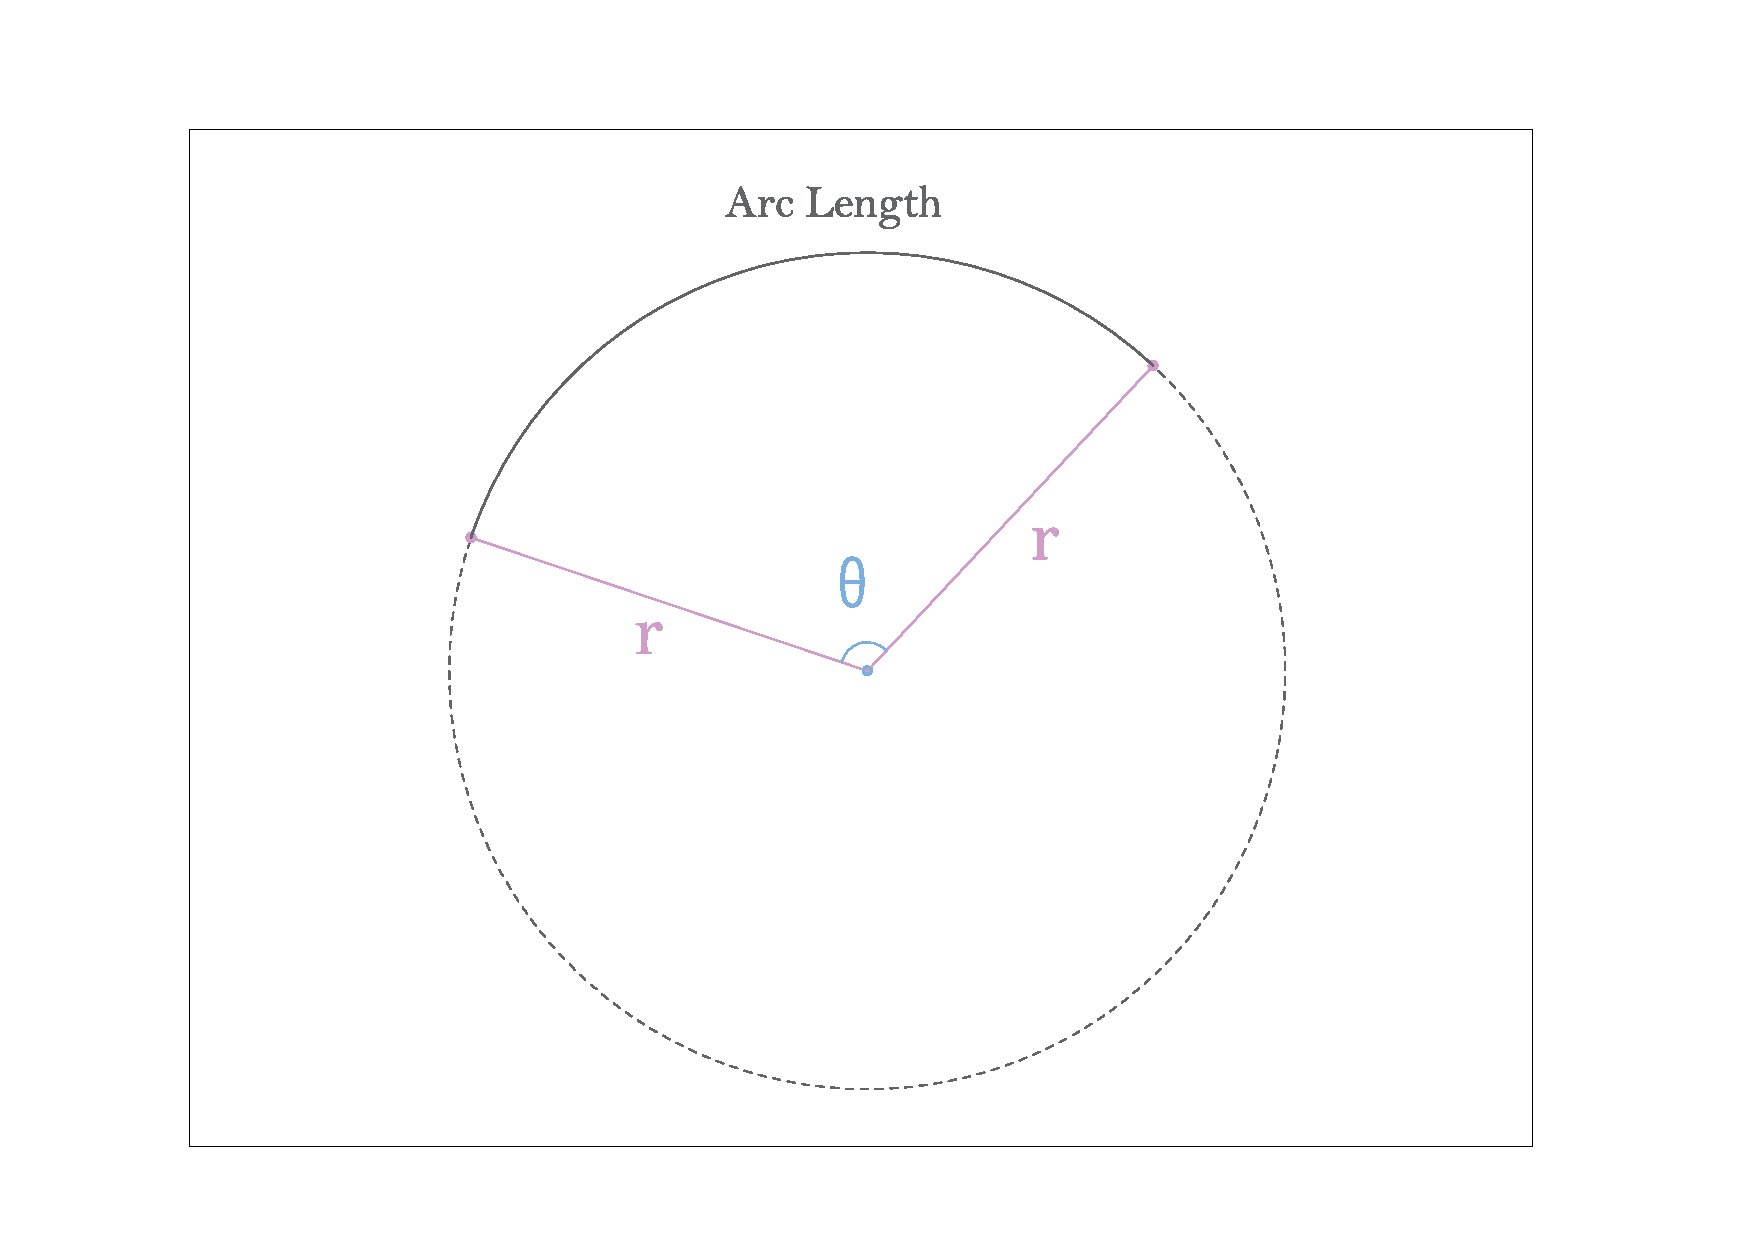
\includegraphics[width=3in,height=3in]{./media/image3.pdf}
%\caption{The arc that the optical flow sensor is tracing }
		%\end{center}
%\end{figure}

%%%%%%%%%%%%%%%%%%%% Figure/Image No: 3 Ends here %%%%%%%%%%%%%%%%%%%%




\paragraph*{Controller}

The voltage controller had some pre-set values. Using the trial and error method, 
initially,  only one of the three variables of the PID controller was changed at 
a time while the others remained set. Regarding the derivative controller, it 
made the system unstable because it made it oscillating and inaccurate. So, 
the best choice was to set the Derivative controller equal to 0. Additionally, 
the combination of changes in the PI controller values decreased the settling 
time, the rise time, the overshoot and the steady state error. As it can be seen 
in the graph bellow, the difference between the initial and the final PID values 
is significant. The overshoot has been eliminated, the rise and the settling 
time have been improved dramatically and the steady state error has an acceptable 
value. Furthermore, it is worth mentioning that if the ratio  \( \frac{ki}{kp} \)  
is great enough (larger than 8) then the response of the system becomes almost 
perfect.
To conclude, by using only a PI controller and by setting P=2.6 and I=27 the 
rover has a stable driving system that does not take a lot of time to stabilise 
its reference voltage (in other words, its reference speed), and most importantly, 
it does not overshoot and oscillate before it takes its reference value. 
These findings can be confirmed by the graph shown in Figure ~\ref{graph:PIDController}.

%%%%%%%%%%%%%%%%%%%% Figure/Image No: 4 starts here %%%%%%%%%%%%%%%%%%%%

\begin{comment}
\begin{figure}[H]
   \centering
   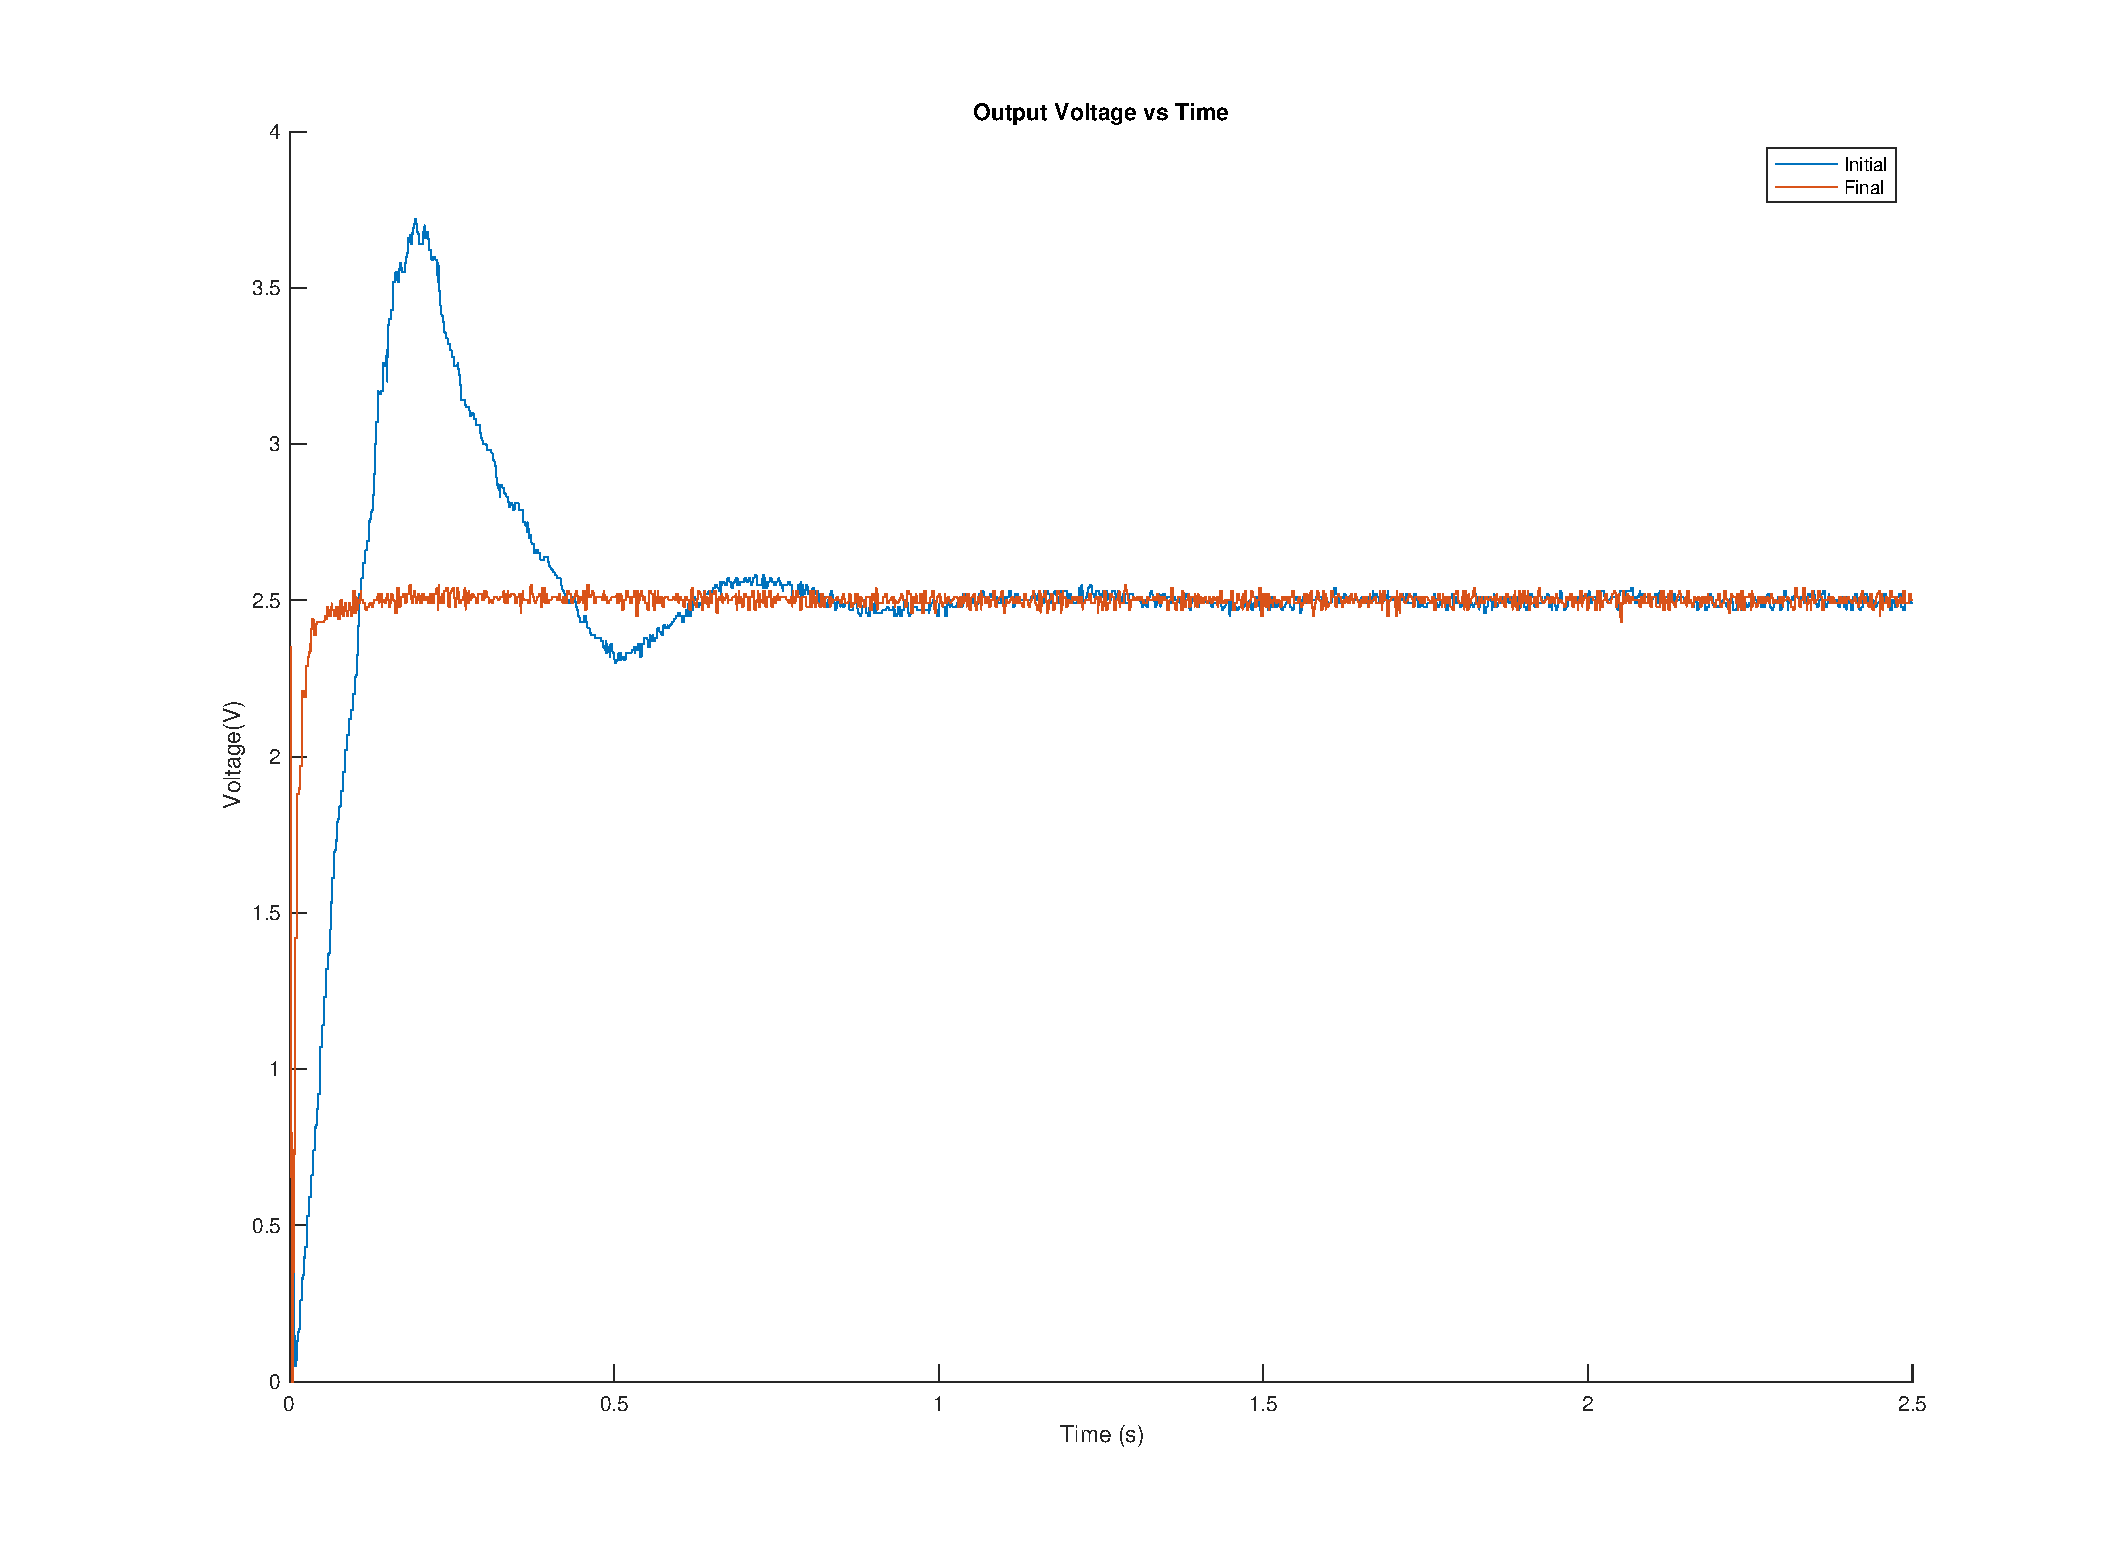
\includegraphics[scale=0.3]{./media/initialvsfinal.eps}
   \caption{Output Voltage vs Time}
   \label{graph:PIDController}
\end{figure}
\end{comment}

\begin{figure}[H]
    \centering
    \begin{minipage}{.4\textwidth}
        \centering
        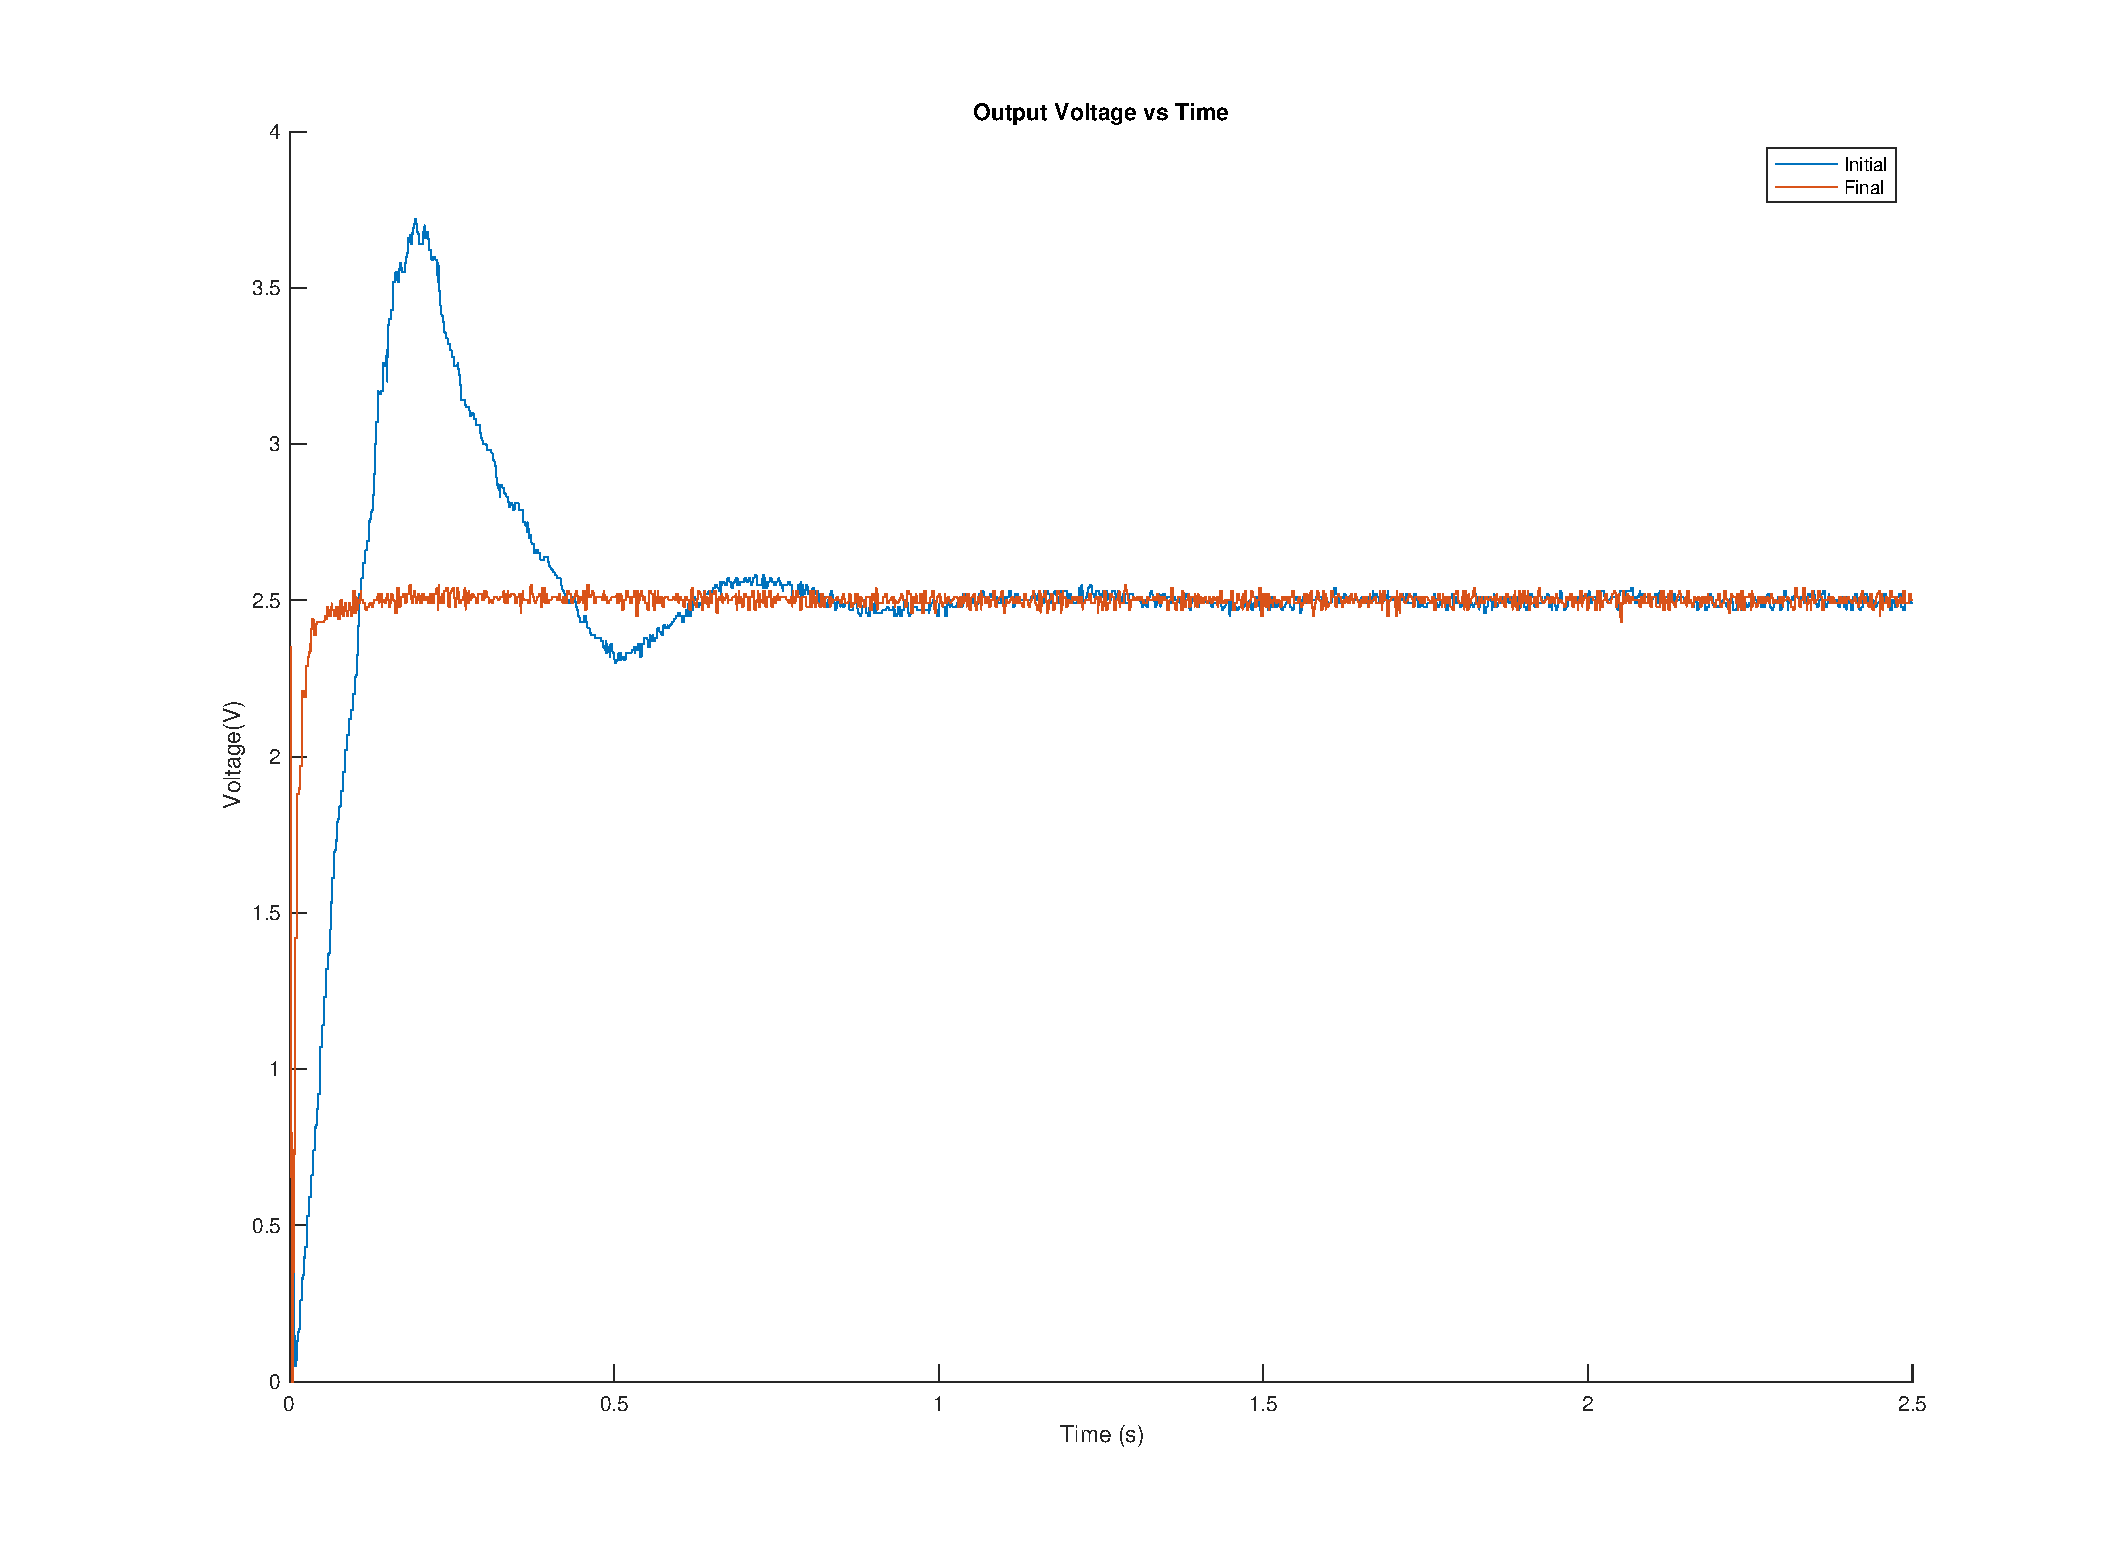
\includegraphics[scale=0.178]{./media/initialvsfinal.eps}
        \caption{Output Voltage vs Time}
        \label{graph:PIDController}
    \end{minipage}%
    \begin{minipage}{.6\textwidth}
        \centering
        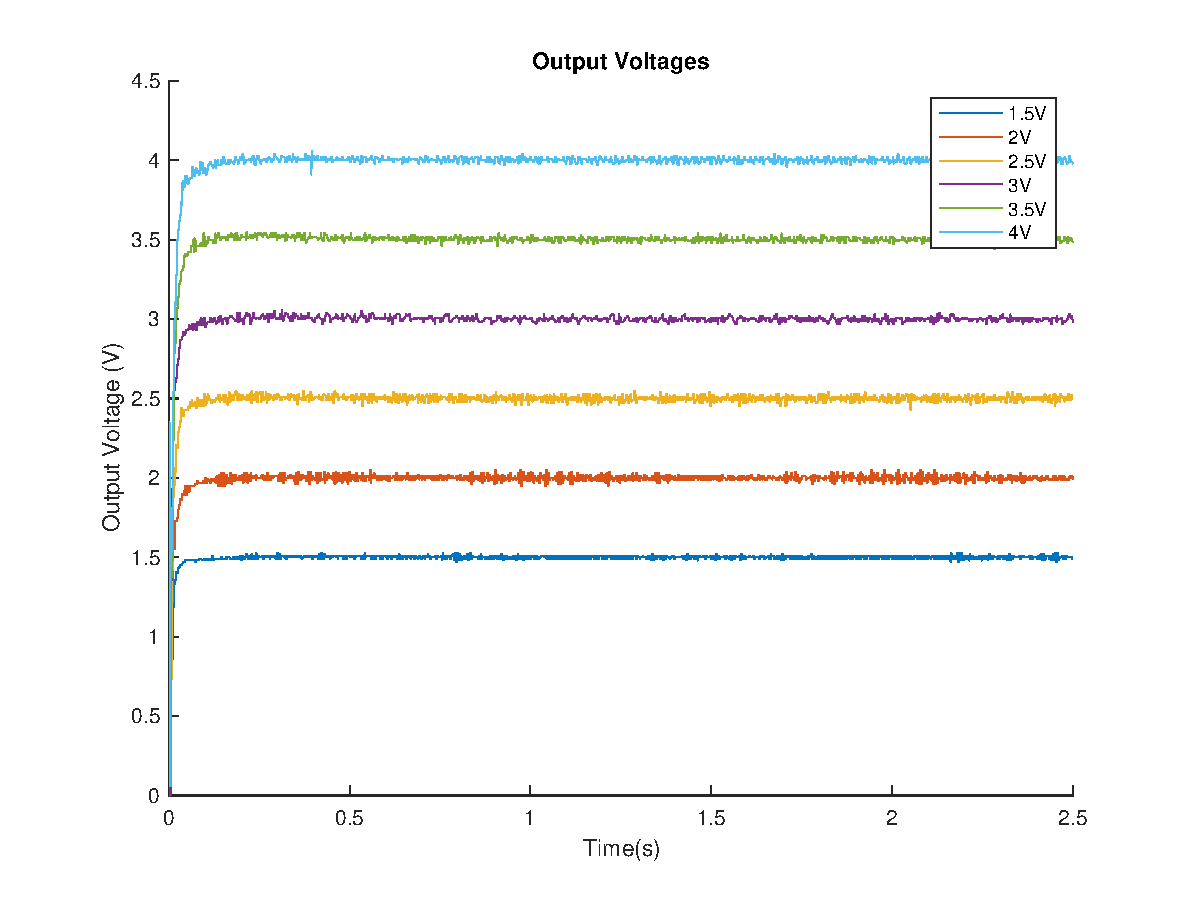
\includegraphics[scale=0.35]{./media/allvoltages.eps}
        \caption{Output Voltages for all Reference Voltages }
        \label{graph:Output Voltages}
    \end{minipage}
\end{figure}

The difference in the system's response is obvious as the system with the final PI values almost instantly reaches its reference value.
The table below is showing the performance of the two PI controllers:


%%%%%%%%%%%%%%%%%%%% Figure/Image No: 4 Ends here %%%%%%%%%%%%%%%%%%%%

%%%%%%%%%%%%%%%%%%%% Table No: 3 starts here %%%%%%%%%%%%%%%%%%%%


\begin{table}[H]
 			\centering
\begin{tabular}{p{0.83in}p{0.99in}p{0.84in}p{0.84in}p{0.84in}}
\hline
%row no:1
\multicolumn{1}{|p{0.83in}}{} & 
\multicolumn{1}{|p{0.99in}}{Overshoot($\%$)} & 
\multicolumn{1}{|p{0.84in}}{Rise time(s)} & 
\multicolumn{1}{|p{0.84in}}{Settling time(s)} & 
\multicolumn{1}{|p{0.84in}|}{Steady State Error($\%$ )} \\
\hhline{-----}
%row no:2
\multicolumn{1}{|p{0.83in}}{Initial} & 
\multicolumn{1}{|p{0.99in}}{48} & 
\multicolumn{1}{|p{0.84in}}{0.143} & 
\multicolumn{1}{|p{0.84in}}{1.25} & 
\multicolumn{1}{|p{0.84in}|}{1.8} \\
\hhline{-----}
%row no:3
\multicolumn{1}{|p{0.83in}}{Final} & 
\multicolumn{1}{|p{0.99in}}{-} & 
\multicolumn{1}{|p{0.84in}}{0.0136} & 
\multicolumn{1}{|p{0.84in}}{0.12} & 
\multicolumn{1}{|p{0.84in}|}{1.6} \\
\hhline{-----}

\end{tabular}
 \end{table}


%%%%%%%%%%%%%%%%%%%% Table No: 3 ends here %%%%%%%%%%%%%%%%%%%%




As it can be seen in Figure \ref{graph:Output Voltages}, using the previous PI values the system 
responds perfectly for all the reference voltages. Also, in the table below are 
given the steady state error for every voltage value. It is really important 
that the system after it has reached its reference value, it does not fluctuate. 




%%%%%%%%%%%%%%%%%%%% Table No: 4 starts here %%%%%%%%%%%%%%%%%%%%


\begin{table}[H]
 			\centering
\begin{tabular}{p{0.73in}p{0.68in}p{0.68in}p{0.68in}p{0.68in}p{0.68in}p{0.69in}}
\hline
%row no:1
\multicolumn{1}{|p{0.80in}}{Voltages(V)} & 
\multicolumn{1}{|p{0.68in}}{1.5} & 
\multicolumn{1}{|p{0.68in}}{2} & 
\multicolumn{1}{|p{0.68in}}{2.5} & 
\multicolumn{1}{|p{0.68in}}{3} & 
\multicolumn{1}{|p{0.68in}}{3.5} & 
\multicolumn{1}{|p{0.69in}|}{4} \\
\hhline{-------}
%row no:2
\multicolumn{1}{|p{0.80in}}{Steady State Error} & %($\%$)
\multicolumn{1}{|p{0.68in}}{1.3} & 
\multicolumn{1}{|p{0.68in}}{2} & 
\multicolumn{1}{|p{0.68in}}{1.6} & 
\multicolumn{1}{|p{0.68in}}{1} & 
\multicolumn{1}{|p{0.68in}}{1} & 
\multicolumn{1}{|p{0.69in}|}{0.75} \\
\hhline{-------}

\end{tabular}
 \end{table}


%%%%%%%%%%%%%%%%%%%% Table No: 4 ends here %%%%%%%%%%%%%%%%%%%%




%%%%%%%%%%%%%%%%%%%% GRAPH No: 5 starts here %%%%%%%%%%%%%%%%%%%%
%\begin{center}
   %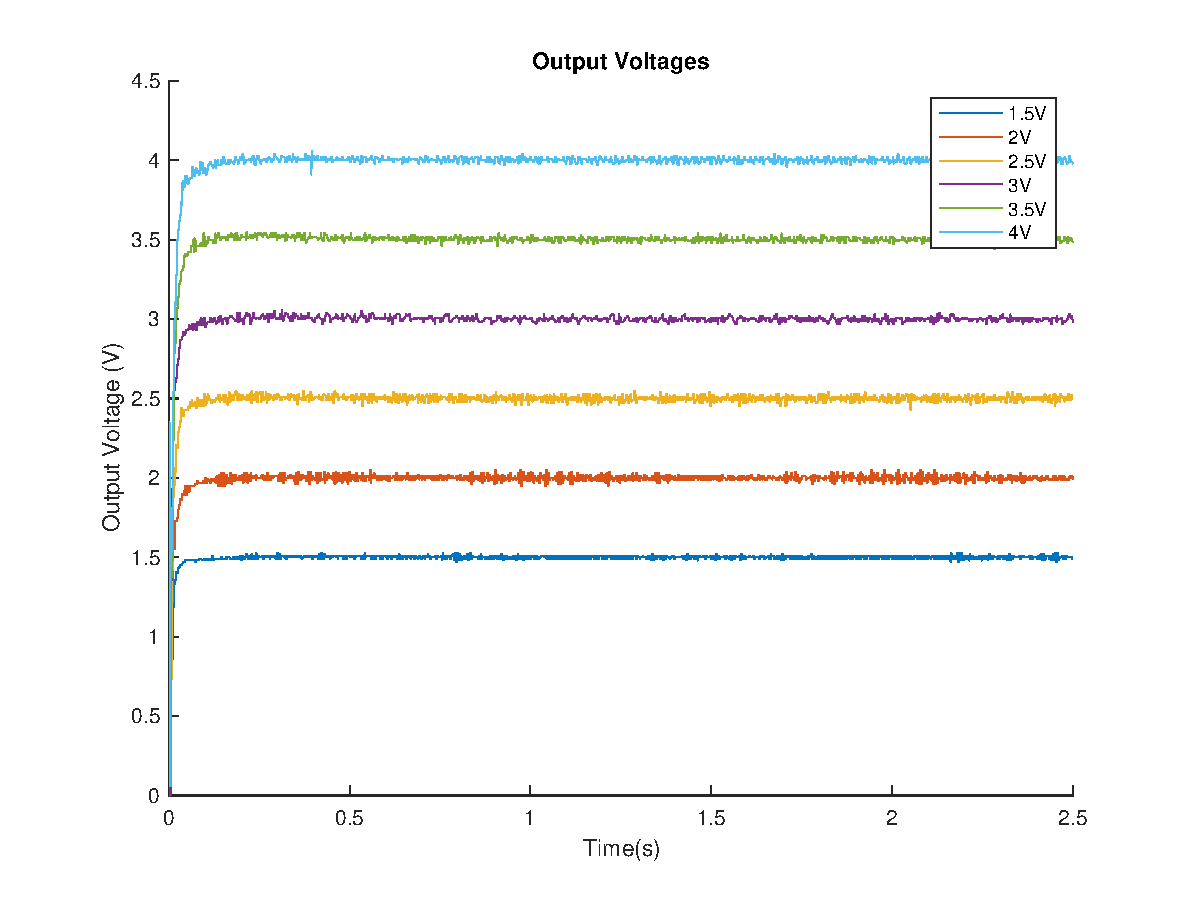
\includegraphics[scale=0.5]{./media/allvoltages.eps}
%\end{center}

\begin{comment}
\begin{figure}
    \centering
    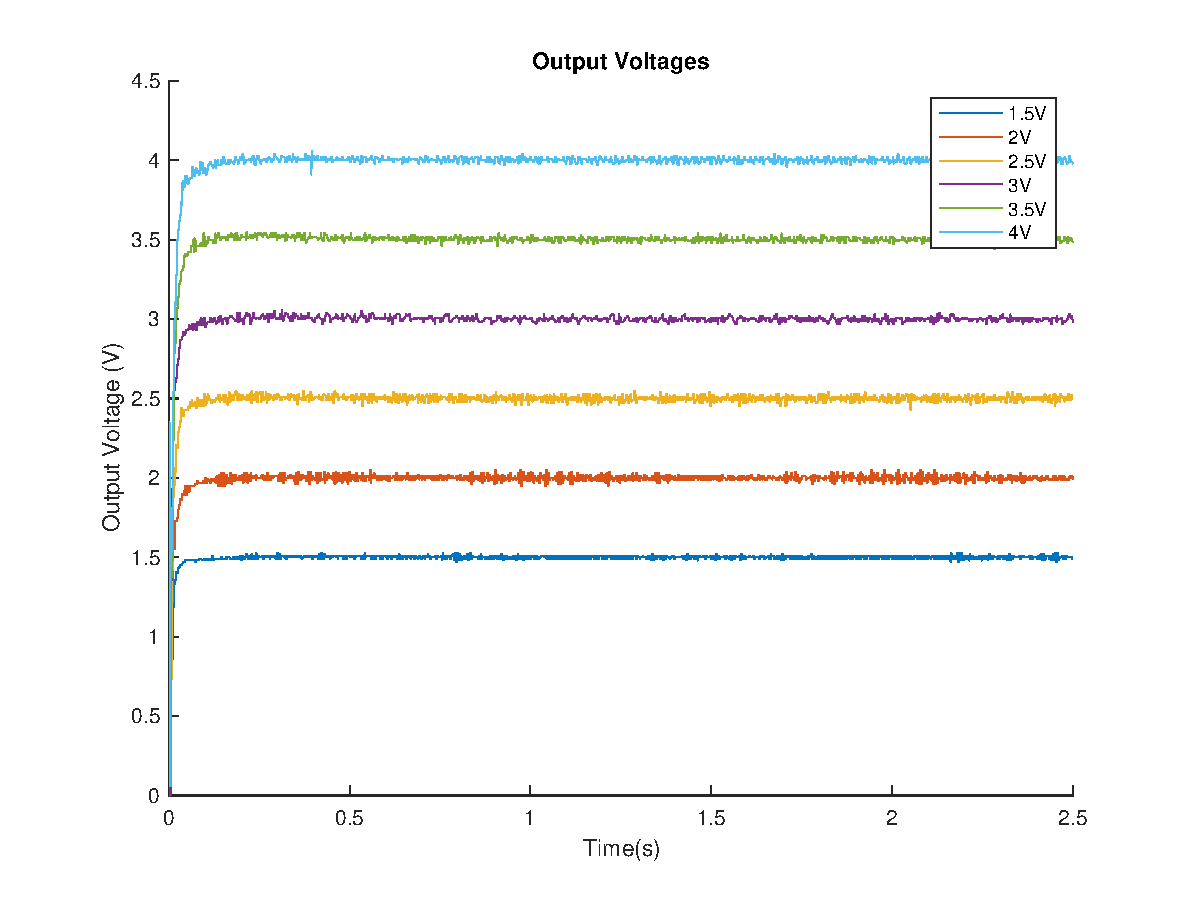
\includegraphics[scale=0.5]{./media/allvoltages.eps}
    \caption{Output Voltages for all Reference Voltages }
    \label{graph:Output Voltages}
 \end{figure}
\end{comment}



%%%%%%%%%%%%%%%%%%%% GRAPH No: 5 Ends here %%%%%%%%%%%%%%%%%%%%
Regarding the Current Controller, it was not tuned because the voltage controller
 interacts with it. Thus, after further testing, making changes to the PI current
  controller gains was not necessary. Finally, the current instantly takes the 
  desired value and it does not oscillate. 





\subsection{Integration}


%Start of energy implementation
\subsection{Energy}

\textbf{SMPS Configuration}
\vspace{10pt} 
\newline
The voltage of the series battery pack is higher than the voltage of the parallel connected
PV panels. The voltage of the PV array must therefore be stepped up before it can be used
for charging. The SMPS must then be operated in boost mode with the
PV panels connected on port B and the battery on port A. Moreover, as the 
SMPS has a max output voltage of 7 V in synchronous boost mode\cite{powerLogbook}, 
it must be operated in non-synchronous mode. To operate in non-synchronous mode switch J1
must be to the left and switch J2 must be to the right. Finally, the on/off switch is 
set to off such that all power comes from the PV array and not from the USB connection 
powering the arduino.

\textbf{Measurements}
\vspace{10pt} 
\newline
Measurements of the circuit currents and voltages are used to track the operation of the
subsystem. When charging the battery the most important measurements are the output voltage,
the cell voltages, and the battery current.

The Arduino can only measure voltages up to 4 V as this is the voltage of its external
reference. However, when using the SMPS in a boost configuration the output voltage will
usually be higher than 4 V and can therefore not directly be measured by the Arduino.
In power labs this issue was overcome through the use of a divide by 3 voltage divider\cite{powerLogbook}.
Using the voltage divider the maximum voltage that can be measured is 12 V, which is still
lower than the expected output voltages when charging the battery. To further divide
the output voltage Vpd further divided by 5/3 using a voltage divider consisting of a 10k
and a 15k resistor. The voltage at this second voltage divider should then be Vout/5, 
which permits the Arduino to measure voltages up to 20 V. The
resistors in the second voltage divider were large, so as to not interfere with the divider
ratio of the first voltage divider. This did however cause a problem as the Arduino draws
some current while sampling, which impacted the operation of the voltage divider. 
To solve this problem the voltage was buffered using an op-amp 
from the Circuits lab before being passed to the Arduino.

The battery cells are configured in series, meaning that the cell voltages will differ from
one another. Every cell voltage therefore needs to be measured individually. Luckily,
the battery boards all have a measurements port specifically for this purpose. By setting
the \emph{RLY} input of a battery board to \emph{HIGH} the cell voltage will appear at the
\emph{MEAS} output. By connecting the \emph{MEAS} output to one of the analogue pins
on the Arduino it is then possible to measure the cell voltage. Note however that when a 
\emph{RLY} input is \emph{HIGH}, the battery cell will not be connected to its power
terminal. If even a single cell is not connected in a series battery, then no current
can flow through the battery. This creates a problem as it means the cells can only 
ever be measured or charged/discharged at a given time. To have the smallest 
impact on the operation on the battery cell voltage measurements should therefore 
be completed as quickly as possible and only be taken when necessary.

The following process was found the be appropriate for measuring the voltage 
of a cell. Firstly, the desired output current is set to 0 mA. If this is not done, 
switching the relay would cause all output current to flow into the capacitor, 
causing the output voltage to spike. Testing showed that after 10 ms the current 
had died down sufficiently for the relay
to be switched on without any large voltage spike appearing. Switching the relay on
takes 6 ms\cite{axicom}. The voltage on the Arduino input then needs about 16 ms to
stabilise after which the voltage can be sampled. Finally the relay can be switched off, which
takes 4 ms, and the measurement process is complete. In total making a measurement takes
about 40 ms. 

To reduce the time spent making measurements it is desireable to measure all cell voltages
at the same time. However, for several reasons this was not found to work in practice. 
Firstly, the design specification adviced against switching multiple relays at the same
time as one might inadvertently create short circuits\cite{energyBrief}. Secondly, measuring
all cells at the same time would take 4 Arduino inputs. Using 4 battery cells the Arduino
already has limited available ports and using 4 of them for cell voltage measurements is not ideal. 
To circumvent both of these issues only one cell voltage is measured at a given time.
The cell voltages do not change very quickly and only need to be measured every couple 
of seconds. It was found to work well if one cell voltage was measured every one second.
As there are 4 battery cells this means that each cell is measured with 4 second intervals.

The current in and out of the battery needs to be tracked to determine the SOC.
However, with the given SMPS configuration the current sensor is on the wrong side of
the SMPS to measure the current flowing into the batteries. The initial attempt at solving
this issue was to connect a 0.5 ohm resistor between the SMPS output and the battery.
By measuring the voltage across this resistor the current into the battery could be
determined. Though initial test gave promising results, an excessively complex circuit
was needed to ensure the sensor worked well for both positive and negative currents.
It was determined that a better solution was to simply calculate the output current
from the input current. When operating at the standard charging current of 250 mA,
the SMPS will be in CCM and the output current can calculated as \( I_{out} = (1 - \delta)*I_{in} \).
For smaller currents however, below about 150 mA, the SMPS might enter DCM. In this case the calculated 
current will be somewhat higher than its true value, which might have an impact on the 
SOC tracking. As such, calculating the output current from the input current is not ideal, 
but is still considered the best option given the available resources. As is discussed 
later the SOC algorithms has methods for correcting itself, which should mean that the
SOC error will not be too large.

\textbf{Controlling the SMPS}
\vspace{10pt} 
\newline
The SMPS is controlled by a dual loop controller, consisting of a fast and a slow loop.
In the design of this dual loop controller the controller from the sample charging code
was used as a starting point\cite{chargeCode}. 

The slow loop in the sample controller consists
of a Moore state machine clocked at 1 Hz, governing the output current. However, as previously
discussed the current setpoint needs to be set to 0 only for a couple of milliseconds when
the cell voltages are being measured. This is not possible with a 1 Hz Moore machine and
as such the slow loop was changed to a Mealy state machine, where the output could change
with the clockspeed of the fast loop. In addition, the slow loop was expanded to also control
the maximum power point tracking.

The fast loop in the sample controller is clocked at 1 kHz and consists mainly of a 
digital PI-controller used to set the duty cycle of the SMPS. As the state machine 
was changed to a Mealy machine, the fast loop was expanded to determine the outputs in
each state. This had the unfortunate side effect of creating timing issues as the code
became more complex than what the Arduino could compute in a millisecond. This issue was
solved by lowering the fast loop clock speed to 500 Hz. This did appear to impact its
performance.
It should also be noted that the PI-gains from the sample code were changed as they did
not work optimally in boost mode. This was done through trial and error.


\textbf{Charging Algorithm}
\vspace{10pt} 
\newline
Constant output voltage was not found to work as it made voltage difference in cells.

\textbf{Balancing}
\vspace{10pt} 
\newline

\textbf{Safety Mechanisms}
\vspace{10pt} 
\newline
In the energy submodule a lot of equipment is used at the limits of what it was designed for.
To prevent damage to the equipment a function was run inside the fast control loop
which every loop checks for abnormal cell voltages and excessive output voltage, input
current and battery current. If any of the measurements are found to be outside the
acceptable range, then the function immediately puts the state machine in the error
state.

\textbf{MPPT}
\vspace{10pt} 
\newline

\textbf{Data Logging}
\vspace{10pt} 
\newline

\textbf{SOC}
\vspace{10pt} 
\newline

\textbf{SOH}
\vspace{10pt} 
\newline

\textbf{Discharging}
\vspace{10pt} 
\newline

\textbf{Final Design}
\vspace{10pt} 
\newline

%End of energy implementation

%End of implementation section









\section{Systems}

\subsection{Control}
 
\subsubsection{Overview of Module and Goals}
The Control module within the context of the rover has one main goal: 
to act as the communication hub between all the subsystems, delivering
the relevant data where it is required to allow for the rover to integrate
as a whole \cite{MarsRoverSpec}. There are a couple of core objectives which must be 
achieved in order to fulfil this role and they are as follows:

\begin{enumerate}
    \item Act as a WiFi Access Point sitting under a router to receive
    commands from the Command subsystem and send data through socket-level communication.
    \item Use a relevant hardware-level data transmission protocol to
    send movement commands to the Drive subsystem and receive data for Command. 
    \item Use a relevant hardware-level data transmission protocol to receive
    the Vision subsystem data.
    \item Connect the Energy subsystem with the rover, sending the relevant data
    to the Command subsystem.
\end{enumerate}

Although the hardware is fixed, the solutions to the outlined problems
above are mostly up to design. It is for this reason that the main challenge
stems from understanding what works best for communication to each subsystem
and more importantly, how to integrate it such that the transmission of data
can be smoothly facilitated through the ESP32.

\subsubsection{Hardware Organisation}

The Control module comprises of two hardware components \cite{BoxContent}: 
the ESP32, a system on chip microcontroller \cite{ESP32Datasheet}, as well as an Arduino adapter
board designed to map some of the available GPIO pins on the ESP32 to an Arduino-like
board \cite{ESP32ArduinoAdapter}.

This hardware was provided by the project organisers and it immediately limits
the tools which can be used, however the wide array of functionality which
this microcontroller can provide through programming the chip allows
for sufficient freedom and capabilities to complete the required tasks. The
GPIO pins are highly configurable when compared to an Arduino-Uno \cite{MicrocontrollerComparison}, as they
are capable of using more data communication through almost any of the pins
via software configuration \cite{ESP32PinOut}. It is low-cost and low-power, 
capable of using WiFi capabilities at 2.4GHz and Bluetooth \cite{ESP32Datasheet} to interface wirelessly
with other devices. Using the Arduino Adapter board \cite{ESP32ArduinoAdapter}, it can sit directly on top of
an Arduino or device with similar pins to directly interface through physical connections. 


\subsubsection{Drive and Control}

\subsubsection{Vision and Control}

\subsubsection{Command and Control}

\subsection{Comms}

\subsection{Vision}


\subsubsection{Hardware Organisation}

The Vision module comprises of two main hardware elements: 
    the Terasic DE10-Lite, a cost-effective Intel MAX 10 based FPGA board 
    \cite{TerasicDE10Web} 
    and the Terasic D8M-GPIO camera package \cite{TerasicD8MWeb}
that interfaces with the FPGA through the onboard GPIO connectors. 

These hardware choices were made by the project organisers, 
but are also sufficient and capable of carrying out the tasks at hand. 
As the FPGA's hardware is configurable, 
it is more flexible than other embedded systems 
that are limited to a general purpose processor,and 
is also able to handle both streaming and processing of high resolution images
without significant compromises on framerate or data speed 
through the use of concurrent operations and dedicated blocks 
for signal processing applications like multiplication.
This particular FPGA is also equipped with a 4-bit VGA output 
which is useful for debugging object detection live, 
and also has a connector for an Arduino Uno R3 shield, \cite{TerasicDE10Web} 
which can be used to interface with the ESP32 used for control.  

In order to perform general purpose operations like
    to configure camera settings
    and to provide a debugging interface,
a Nios\textsuperscript{\textregistered} II/f "Fast" soft core was instantiated on the FPGA. 
Alternatively, to implement more advanced image processing algorithms
or to reduce other hardware components in the system like the multiple Arduinos, 
a FPGA with a hard core connected via PCIe, 
known as a FPGA System-On-Chip (FPGA SoC) \cite{FPGASoC} could be used, 
which would provide both the advantages of having reconfigurable hardware,
a more capable general purpose processor and a higher bandwidth limit. 

\subsubsection{Image Capture \& Processing Stream}

The image capture and buffering is based on a starter project provided
by Terasic Inc for the D8M Camera module that was modified by Dr Edward Stott 
\cite{EEE2Rover} and provided to us for this project. The system makes use of 
several IP components from the Intel Video and Image Processing Suite,
namely the Clocked Video Output and Frame Buffer Core. The system is compromised
of several modules, that take the raw data from the camera in Bayer filter form\cite{TerasicD8MWeb},
transform it into RGB video packets, buffer the frames to allow camera and output
to run at different frame rates, process the image data and convert the video 
data to serial data for output over VGA.\cite{EEE2Rover} As this system and its 
corresponding documentation is openly available, the implementation outside of 
the image processor will not be described in more depth, interested readers can 
consult the provided repository and starter project for reference. 

\subsubsection{Image Pre-Processing Module}

The challenge for this rover was to detect different coloured ping-pong balls as
obstacles and relay the information about these obstacles to the control module. 
The provided ping-pong balls came in 5 different colours - pink, orange, light 
blue, grey and green. As these colours cover a wide range of the colour spectrum
and even overlap with each other (orange and pink, blue and grey), it was thought 
to be necessary to do some preprocessing on the incoming image from the camera 
to ensure optimal colour detection for object detection.  
 
%Maybe add Image of all the balls here. 


The initial design and implementation of this image processing algorithm involved
a transform from the RGB (Red, Green, Blue) colour space to the HSV (Hue, 
Saturation, Value) colour space, and pixel based classification to detect large
areas of the necessary colours.  HSV has been shown to be a better colour space
for image processing tasks like colour segmentation in road sign detection for 
autonomous driving as it is invariant to illumination changes unlike the RGB 
space.\cite{ali2013performance} As the task at hand here is similar, a transformation
from the RGB space to the HSV space is applied. 

HSV is traditionally expressed as three values ranging between 0-360\degree\  
for hue, and two values between 0 and 1 for saturation and value.\cite{10.1145/965139.807361}
As floating point calculations in SystemVerilog are computationally expensive, 
and also introduce a layer of unnecessary complexity, the conversion was adjusted
to express all three values in terms of an 8 bit integer ranging from 0-255. The
algorithm for conversion from 8-bit RGB integers is presented mathematically:

\begin{multicols}{3}
    \noindent
    \begin{align*}
        M &= \max(R, G, B) \\ \\
        m &= \min(R, G, B) \\ \\
        C &= M-m 
    \end{align*}
    \begin{equation*}
        H = \begin{cases}
            M = R, & 0 + \frac{43 \times (G-B)}{C} \\
            M = G, & 85 + \frac{43 \times (B-R)}{C} \\
            M = B, & 171 + \frac{43 \times (R-G)}{C} \\
            M = 0, & 0 \\
            C = 0, & 0
        \end{cases} 
    \end{equation*}
    \begin{align*}
        S &= \begin{cases}
            M = 0, & 0 \\ C = 0, & 0 \\ \text{else} & \frac{255\times C}{V}
        \end{cases} & \\ \\
         V &= M  
    \end{align*}
\end{multicols}



Although the inclusion of a divide operation was undesirable as it does not 
translate well to hardware implementations, it was unavoidable with hue being 
obtained by dividing the difference of two components by the chroma value. This 
module was then implemented using two pipelined 3 cycle divider from the Intel IP
megafunction library for the hue and saturation value calculations.  

The YUV colour space was also considered as a option for conversion as it also
separates colour into 3 components - one for luma and two chrominance components.
This would also make it invariant to illumination changes. The transform from RGB
to HSV is also more suited to hardware as it is a linear transform requiring only
multiplication. However, as it cannot represent the full RGB spectrum and is 
limited in what colours it can represent, the decision was made not to use it.    


\subsubsection{Image Object Detection Algorithm}

There are several common approaches to object detection, with the two most 
prominent being the use of classic Computer Vision algorithms like the Canny edge-
detection technique and Hough transforms or the more recent use of convolutional
neural networks (CNN) and deep learning to perform object detection through a 
combination of layers that perform convolution, pooling and fully connected layers. 
According to \cite{DBLP:journals/corr/abs-1806-01683}, CNNs have in recent years 
become the de-facto standard for machine vision applications such as object 
classification, object detection and object segmentation; but as there is a desire 
for more performant and power- efficient systems, there has been a shift to 
using dedicated hardware tailored to the operations used for CNNs. There was a 
deep interest from the technical lead for the Vision module for this and he spent 
a bit too much time researching this field, and was left with less time for the 
project. There were far too many challenges for implementing a CNN within the 
current project with key issues being the system is a real-time system that 
processes video data pixel-by-pixel in a fixed order with most CNNs for object 
detection working with multiple pixels in different locations Simultaneously and
a lot of previous work on the subject is on FPGAs being used as accelerators for 
CNNs running on hard cores rather than standalone embedded systems as seen in \cite{DBLP:journals/corr/abs-1806-01683}
. This was also a challenge for implementing traditional computer vision 
algorithms on the FPGA,  the same problem of not being able to access random 
pixels exists. 


\subsubsection{Object Location Calculations}

With the bounding boxes obtained from the Verilog module, the coordinates of the
bounding box for each colour is sent to the NIOS II processor using a FIFO buffer.
The calculations for how far away the object is and it's relative position in 
comparison to the camera module was are done on the NIOS II processor. 

There are multiple ways to calculate the location of a 3D object in space on a plane
with some ways being more precise than others. 

%TODO!! Add survey of other potential algorithms and why this one was chosen. 

As the testing environment for the rover was ideal with the camera in a fixed 
position and the testing surface being completely level, the initial algorithm 
for the mapping between pixel coordinates and real world x-y coordinates relative
to the camera was based on the following form: \begin{align*}
    x & = A_x m^2 + B_x n^2 + C_x mn + D_x m + E_x n + F_x \\
    y & = A_y m^2 + B_y n^2 + C_y mn + D_y m + E_y n + F_y  
\end{align*} By taking a picture of multiple balls in different locations and 
measuring the actual corresponding mapping distance and the pixel locations, the
coefficients can be found by solving the matrix equation: $$
    \begin{bmatrix}
        m^2_1 & n^2_1 & m_1n_1 & m_1 & n_1 & 1 \\
        m^2_2 & n^2_2 & m_2n_2 & m_2 & n_2 & 1 \\
        .     & .     &    .   &  .  & .   & . \\
        m^2_i & n^2_i & m_in_i & m_i & n_i & 1 \\  
        .     & .     &    .   &  .  & .   & . \\
        m^2_N & n^2_N & m_Nn_N & m_N & n_N & 1  
    \end{bmatrix}
    \cdot
    \begin{bmatrix}
        A_x & A_y \\
        B_x & B_y \\
        C_x & C_y \\
        D_x & D_y \\
        E_x & E_y \\
        F_x & F_y
    \end{bmatrix}
    =
    \begin{bmatrix}
        x_1 & y_1 \\
        x_2 & x_2 \\
        . & . \\
        x_i & y_i \\
        . & . \\
        x_N & y_N
    \end{bmatrix}
$$ where the pixel locations are represented by \((m,n)\) and the physical locations on
the plane are represented by \((x,y)\). Initially 6 samples were taken to calculate 
the coefficients, but as more measurements were taken to verify the method, they
were also added to the list of samples to improve the accuracy of the algorithm.
These calculations for the coefficients were carried out in MATLAB, and then 
implemented in C on the Nios\textsuperscript{\textregistered} II processor. 

This method is satisfactory in its performance, with a worst case error of \(\pm5\unit{cm}\)
in difference between calculated position and actual position. For the rover's 
path finding algorithm, this is a value that is easily taken into account and as
multiple measurements of the ball are taken, the actual position can be refined 
and accurately determined by taking the average of multiple readings in the 
Command module in the server. 

The Nios\textsuperscript{\textregistered} II processor does not include floating point hardware by default, but as 
this algorithm requires floating point calculations as some of the coefficients 
tend to be very small, and this algorithm is run for each set of colours, it was
prudent to include hardware support for single precision floating point adds 
and multiplications. This was done by adding a module from Intel's IP catalogue 
for custom floating point instructions, this reduces the amount of cycles 
necessary to carry out a floating point multiplication to 4 cycles using a single
instruction and a floating point add to 5 cycles\cite{NiosIICustomInstruction}.
If this hardware was not used, it would be implemented using software, and hence
would take multiple instructions and more hence more cycles. 

This algorithm's performance is satisfactory in the current testing environment, 
but if tested on a surface with changing gradients or elevated objects, this algorithm
would be inaccurate due to it's inability to take into account objects on the real
world z-axis (i.e. the height of an object relative to the plane).  


the best implement an algorithm that could take into account the location 
and shape of the ball, as a purely colour based algorithm would be unable to 
differentiate other objects in view of the camera and confuse them with the ball, 
for example, the sky and the light blue ball would be seen as one object.


\section{Evaluation and Conclusion}

\section{Project Management and Organisation}
%Also had frequent teams meetings and used WhatsApp
As this project was carried out remotely
with contributors located in different countries, 
it was important to have a good framework for communication and management. 
For direct communications between the team, WhatsApp was used for short texts, 
and Microsoft Teams was utilised for calls as its screen-sharing functionality 
was useful for helping to debug errors. 

The main tool used for written communications and management was Git + GitHub.
As the codebase was incredibly complex, 
involving many different libraries and with each submodule being capable as a
standalone project, it was vital to have a version control system in place. 
Being able to keep a history of commits and changes made to a project was useful,
especially when trying to track down the origin of a bug and what caused it. 

The team also made use of GitHub Issues to track progress and accountability in 
the initial design phase. A thread was opened for each submodule to show what 
the lead for that submodule had been doing and potential avenues of achieving 
their goals. This was beneficial both for the leads to keep track of their 
research, but also allowed other members to contribute to other submodules 
by adding comments and voicing their thoughts. GitHub Issues were also linked 
directly to commits in the codebase to allow for a more in-depth explanation and
reasoning with context for a commit than what is allowed in the commit message 
area. 

By way of using GitHub, the team also made use of GitHub's Actions, which allow 
for automated workflows to be run on certain events like a commit or a push for 
continuous integration. An Action was designed for the writing of this report
that compiled the \LaTeX document and produced a PDF. 

Simultaneously, a Gantt chart was maintained to keep track of progress and is 
available for viewing under the maintained GitHub repository linked in the Appendix.

%TODO #7!
\section{Intellectual Property}
Intellectual Property (IP) is a complex topic that has financial, technological, 
and moral significance when developing products or inventions. In short, IP rights are what
lets companies, inventors and creators prevent other people from using their work\cite{perea}.
Many types of IP rights exists including copyrights, trademarks, design rights and patents.  

In the context of our design project, there are sections within IP which are less applicable than others. 
These include trademarks, as no brand is being developed, and design rights, as the rover's physical design has
been provided by the college and will not be significantly altered by students. Note however,
that as the college has created the rover design, it owns the design rights and could stop students
from using its appearance if desired, but would probably fail to obtain legal orders for it as the design
has been "publicly" circulated and freely provided.
Patenting is a vital step which should be encouraged for inventors to apply their negative rights and 
protect themselves from any infringement which seeks to use their original inventive work without permission. 
There are clear guidelines in place to determine what constitutes a patent and unfortunately, 
this is not the case for our rover. By no means is it a novel idea; all the technology being 
applied to the rover, like the hardware, communication protocols, vision algorithms and functionality 
have all been explored in depth and this could not be clearer when we look at the countless missions, 
development and papers that have been written for true Mars Rovers like Perseverance. 
Although there is a case to be made for industrial applicability, this first requirement being 
violated immediately nullifies the possibility of a patent. What is relevant is copyright as 
the combination of software algorithms being applied could be considered complex enough to assert 
copyright as it is original expression. However, as the Arduino and its libraries are under the GNU General 
Public License \cite{ArduinoLicense}, an open-source license, users need to follow the same license 
when using these libraries and we would hence be restricted to an (L)GPL license as well. A more complex 
situation is the system that is running on the FPGA, although all components are available for testing 
in what is known as the Intel FPGA IP Evaluation Mode, any commerical use of the IP would require a   
license to be bought from Intel\cite{IntelEvalMode}. There are few individual modules written in SystemVerilog that could be copyrighted, 
like the Image processing module and the image transfer over SPI module, if the FIFO and divider components were replaced
with either open-source/self-designed modules. 

\begin{comment}
This is just a draft, feel free to edit, add, remove, and change what you want.
Currently at 264 words
\end{comment}
\begin{comment}
Could link stuff about how we are using Intel IP in the FPGA, as well as things
like licencing and how some companies make their entire business based on it,
like Arm, hence ethically it is important to maintain standards and rules for IP
through the use of legislation and governmental regulatory authorities. 
\end{comment}
\begin{comment}
A lot of the technologies that we have used in this project is probably covered
by a patent.
\end{comment}
\begin{comment}
Could also talk about how some of the Libraries for the Arduino are open source
and the benefits that those bring to development in projects like these which
are not funded and the benefits of open source in general maybe?
\end{comment}

 
\newpage

\printbibliography[
heading=bibintoc,
title={References}
]


\newpage
\begin{appendices}


\chapter{Appendix 1: Circuit Diagram of the Energy Submodule}
\begin{figure}[H]
    \centering
    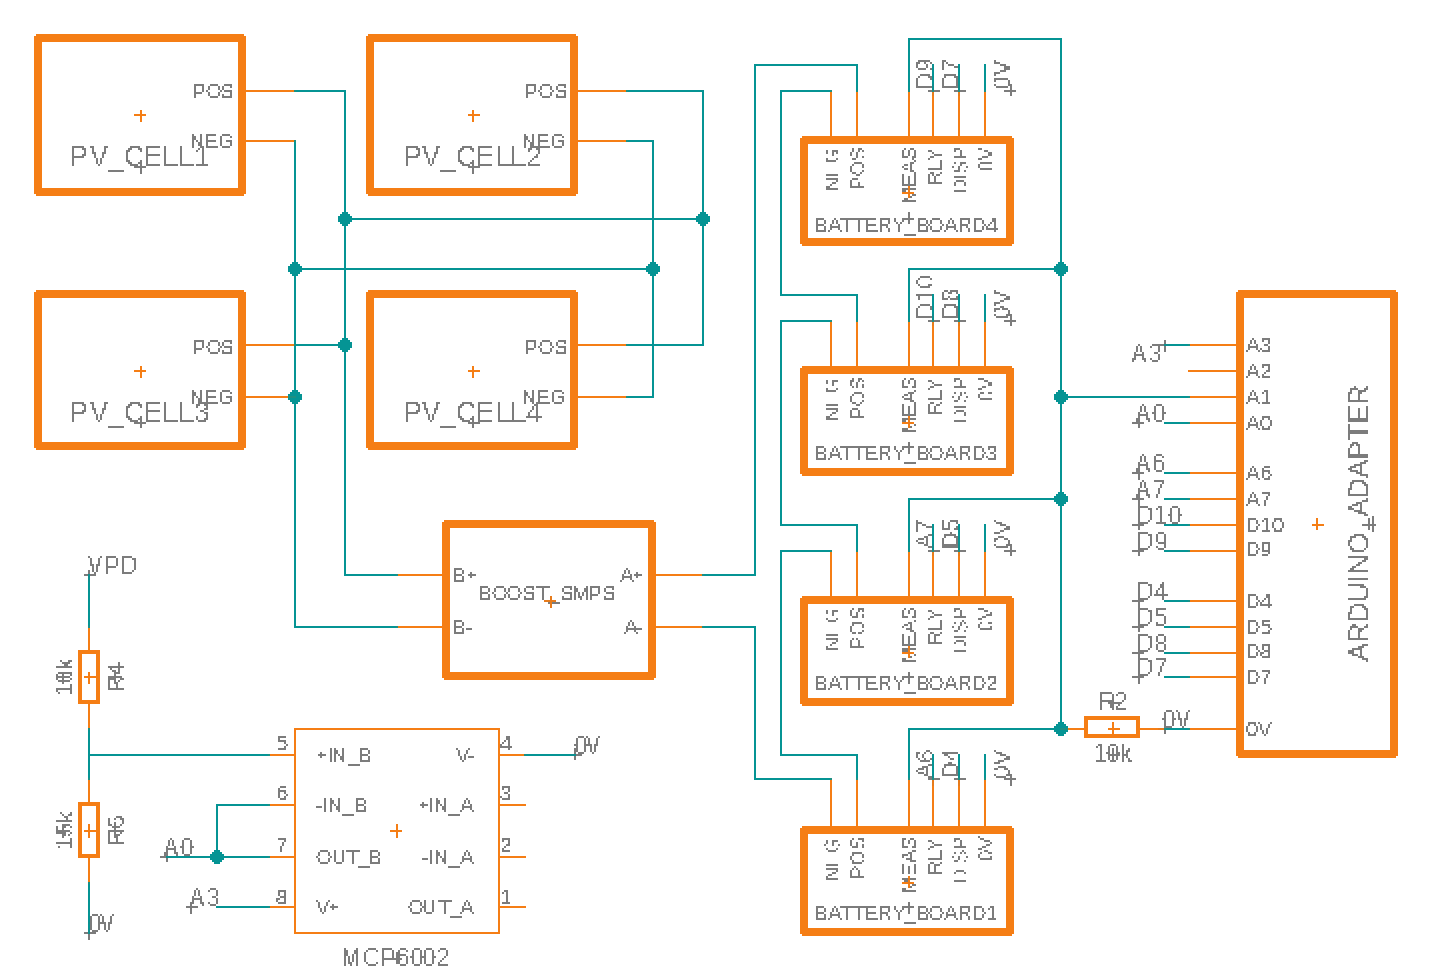
\includegraphics[width=\textwidth]{Circuit_Diagram.png}
    \label{fig:circuitDiagram}
\end{figure}





\end{appendices}

\end{document}